\documentclass[11pt]{article}
\usepackage[margin=1in]{geometry}
\usepackage{amsmath,amssymb}
\usepackage{booktabs}
\usepackage{hyperref}
\usepackage{graphicx}
\usepackage{xcolor}
\usepackage{tikz}
\usetikzlibrary{arrows.meta, positioning, shapes.geometric, calc}
\usepackage[numbers]{natbib}
\usepackage{enumitem}
\usepackage{listings}
\newcommand{\pninetyfive}{\ensuremath{\mathrm{p95}}}
\newcommand{\pninetynine}{\ensuremath{\mathrm{p99}}}
\newcommand{\slo}{\ensuremath{\mathrm{SLO}}}
\newcommand{\etal}{\textit{et al.}}

\title{Spec-Driven, SLO-Aware Agents on a Single GPU}
\date{}
\begin{document}
\maketitle

\usepackage{tikz}
\usetikzlibrary{arrows.meta, positioning, shapes.geometric, calc}

\section{Introduction}

LLM agents are moving from prototypes to production services.
In production, an agent is not merely a model that produces text---it is a \emph{contracted component} in a larger system that must (i) emit \emph{structured outputs} that downstream software can parse and validate, (ii) remain \emph{faithful} to provided context (retrieved passages, records, logs, or tool outputs), and (iii) satisfy latency \emph{service-level objectives} (\slo s), where users experience tail latency (\pninetyfive/\pninetynine), not averages~\citep{dean2013tail}.
When these requirements are violated, failures are not cosmetic: malformed JSON breaks ETL and dashboards; subtly unsupported claims about metrics trigger incorrect business actions; heavy-tailed response times collapse throughput and user trust.

These requirements are especially acute in the increasingly common \emph{single-GPU deployment} regime:
teams run open-weight models behind OpenAI-compatible local servers (e.g., LM Studio, Ollama, vLLM) to control cost and keep sensitive data on-premise.
Single-node deployments have tight resource envelopes and sharply visible tail behavior under load, yet they still face the same production realities as cloud deployments: strict schema contracts, tool-call correctness, and faithfulness to internal data.
In practice, many teams will accept slightly higher latency to enforce correctness, but they still need predictable \pninetyfive/\pninetynine bounds to avoid operational instability.

Existing work addresses parts of this problem in isolation.
Systems research and serving runtimes target throughput and tail latency for Transformer inference~\citep{kwon2023vllm,zheng2023sglang,deepspeedFastGen,agrawal2024sarathi}, but typically treat the model as a black box producing unconstrained text.
In parallel, providers and open-source libraries offer \emph{structured output} and \emph{constrained decoding} modes (schemas, grammars) that drastically improve syntactic validity, as reflected in recent benchmarks~\citep{geng2025jsonschemabench,letmespeakfreely,structuredRAG}.
However, the community lacks a portable, backend-agnostic framework that ties these capabilities to the behaviors practitioners actually gate on in production:
schema correctness \emph{and} task accuracy \emph{and} faithfulness \emph{and} tool-call reliability \emph{and} stability \emph{and} tail-latency \slo s---especially for single-GPU local stacks.

We introduce \emph{SpecSLOEval}, a contract-first, \slo-aware agent evaluation and serving framework designed explicitly for single-GPU OpenAI-compatible endpoints.
SpecSLOEval treats JSON Schemas (and tool argument schemas) as first-class contracts, compiles them into backend-specific structured decoding modes where possible, hardens outputs via bounded validation-and-retry, and evaluates configurations using a single, versioned criteria file (\texttt{criteria.yaml}) that defines metric families, thresholds, and lexicographic gates.
In P1, we focus on establishing a stable baseline and measurement methodology; the same metrics are designed to be reused as reward components and constraints in subsequent PPO/GRPO-style optimization~\citep{schulman2017ppo,grpo,dettmers2023qlora}.

\paragraph{Contributions.}
This paper makes three contributions:

\begin{itemize}[leftmargin=12pt]
    \item \textbf{Contract-first, single-GPU agent harness.}
    We present a spec-driven agent stack for OpenAI-compatible local servers that enforces structured output contracts via backend-native structured outputs when available, and otherwise via explicit schema validation, canonicalization, and bounded retry with an auditable error taxonomy.
    \item \textbf{A unified evaluation protocol with explicit gates.}
    We formalize a portable evaluation suite configured by a single \texttt{criteria.yaml} that defines metric families (structure, accuracy, faithfulness, tools, stability, \slo) and a strict lexicographic gating policy.
    We instantiate P1 on three representative task families aligned with the criteria file: intent classification (CLINC), grounded QA with explanations (HotpotQA), and tool-call episodes.
    \item \textbf{A measurement study of contract enforcement under tail \slo s.}
    We benchmark unconstrained decoding versus structured-output and spec-driven modes on single-GPU backends, reporting the joint frontier between structural validity, task success, faithfulness, and \pninetyfive/\pninetynine latency.
\end{itemize}

\paragraph{Paper organization.}
Section~\ref{sec:background} reviews related work in LLM serving, constrained decoding, and agent evaluation.
Section~\ref{sec:problem} formulates contract-first, \slo-aware serving as constrained optimization over configurations.
Section~\ref{sec:method} details our spec-to-decoder compilation and serving-time hardening (validation-and-retry, budgeted selection).
Section~\ref{sec:eval-framework} presents the evaluation framework and test families, including faithfulness scoring and trajectory checks.
Section~\ref{sec:experiments} reports single-GPU experiments and decoding-mode comparisons.
Section~\ref{sec:discussion} discusses limitations and future directions.

\section{Background and Related Work}
\label{sec:background}

Our work connects four lines of research and practice: (i) tail latency and LLM serving systems, (ii) structured outputs and constrained decoding, (iii) automated evaluation of faithfulness and reliability, and (iv) agent evaluation workflows used in production.
We review each and highlight the specific gap addressed by SpecSLOEval.

\subsection{Tail Latency and LLM Serving}

Users experience tail latency, not mean latency.
Dean and Barroso’s “The Tail at Scale”~\citep{dean2013tail} explains why small fractions of slow requests dominate perceived quality and limit system scalability.
Transformer serving inherits and amplifies tail behavior due to variable output lengths, batching dynamics, and expensive decoding.

Recent LLM serving systems target throughput and tail latency via optimized KV-cache management, batching, scheduling, and kernel-level improvements.
vLLM proposes PagedAttention and continuous batching~\citep{kwon2023vllm}.
SGLang emphasizes efficient execution of structured LM programs and scheduling~\citep{zheng2023sglang}.
DeepSpeed-FastGen and attention-kernel advances reduce inference overhead~\citep{deepspeedFastGen,dao2023flashattention2,prabhu2024vattention}.
Sarathi-Serve analyzes throughput--latency trade-offs and scheduling under realistic traffic~\citep{agrawal2024sarathi}.
These systems are essential for performance, but they generally assume unconstrained text generation and do not treat \emph{output contracts} or \emph{semantic faithfulness} as first-class service objectives.

\textbf{Gap:} serving work optimizes inference mechanics and tail latency but does not define how to measure (or enforce) contract correctness, tool reliability, or faithfulness alongside tail \slo s.
SpecSLOEval targets exactly this joint measurement surface on single-GPU stacks.

\subsection{Structured Outputs, Grammars, and Contract-First Decoding}

Many agent integrations require structured outputs: JSON reports, typed objects, or tool-call payloads.
Providers and local runtimes increasingly expose structured-output interfaces (e.g., OpenAI-style schemas and tool calling; local OpenAI-compatible servers such as LM Studio and Ollama), and open-source libraries compile schemas into decoding constraints (e.g., grammar-based or schema-based constrained decoding).

Benchmarking work shows that constraints substantially improve syntactic validity.
JSONSchemaBench~\citep{geng2025jsonschemabench} systematizes schema-following tasks; analyses of format constraints and structured RAG highlight that constraints can reshape generation behavior beyond syntax~\citep{letmespeakfreely,structuredRAG}.
However, most structured-output evaluations stop at “does it parse / validate,” and do not connect constrained decoding to \emph{service-level} concerns: how constraints interact with tail latency under load, how often retries occur, or whether improved syntax correlates with improved semantic correctness.

\textbf{Gap:} constrained decoding is typically evaluated as a formatting primitive, not as part of an end-to-end agent service that must satisfy contracts \emph{and} faithfulness \emph{and} tail \slo s.
SpecSLOEval evaluates structured output modes in exactly that end-to-end setting.

\subsection{Automated Evaluation of Faithfulness and Factuality}

Faithfulness---whether an output is supported by the provided context---is a central production risk for analytics and RAG-style agents.
RAGAS~\citep{es2023ragas} popularized LLM-as-judge scoring for faithfulness and answer relevance in retrieval-augmented settings.
Atomic-fact approaches decompose outputs into fine-grained claims and score support per claim, improving interpretability and surfacing subtle hallucinations~\citep{atomicFacts2024}.

LLM-as-judge methods are powerful but imperfect.
Studies document judge bias and sensitivity to prompt framing and verbosity, motivating careful calibration and auditability~\citep{llmjudgebias}.
For production use, judge outputs must be treated as \emph{signals} that are logged, inspected, and complemented with task-grounded checks.

\textbf{Gap:} faithfulness evaluation is often bolted on after generation and is rarely integrated with structured-output contracts, tool traces, stability, and latency \slo s in a single harness.
SpecSLOEval integrates judge-based faithfulness scoring as one metric family in a strict, auditable gating pipeline.

\subsection{Agent Evaluation Frameworks in Practice}

Production agent stacks increasingly adopt evaluation pipelines: golden sets, rubric scoring, trajectory inspection, and regression tests.
Cloud ecosystems (e.g., Google’s ADK and Vertex AI evaluation guidance) emphasize both final answer quality and trajectory quality (tool use, error handling) and provide templates for evaluation workflows.
These resources are operationally valuable, but they are often platform-tied, assume managed model hosting, and under-specify how to combine schema contracts, tool-call validity, faithfulness, stability, and tail-latency constraints into a single, portable protocol.

\textbf{Gap:} existing production frameworks describe the \emph{idea} of agent testing but do not provide a backend-agnostic, single-GPU-friendly criteria-driven harness that makes contracts and tail \slo s first-class.
SpecSLOEval provides this explicit criteria layer (\texttt{criteria.yaml}) and a repeatable execution harness.

\subsection{Single-GPU Local Serving and Open-Weight Models}

Single-node deployments---a workstation GPU (e.g., RTX~4090) or laptop accelerators (Apple M-series)---are common for privacy, cost predictability, and rapid iteration.
Local OpenAI-compatible servers (LM Studio, Ollama) and high-throughput runtimes (vLLM) make such deployments practical.
What is missing is a standardized way to evaluate these stacks as \emph{services}: not just average latency, not just “does JSON parse,” but the joint behavior under contracts, tool usage, faithfulness, stability, and tail \slo s.

\textbf{Gap:} the ecosystem provides runtimes and knobs, but not an end-to-end evaluation protocol that treats structured contracts and tail \slo s as co-equal first-class citizens.
This motivates our problem formulation in Section~\ref{sec:problem}.

\section{Problem Formulation}
\label{sec:problem}

Figure~\ref{fig:agent-context} sketches the single-node setting we target.
A generic commercial agent sits between upstream requesters (users, batch jobs, or other services) and downstream consumers (dashboards, workflows, humans).
For each request, the agent receives unstructured and structured context (documents, logs, records, prior turns), may call tools (APIs, databases, services), and is expected to emit \emph{structured outputs} such as JSON reports, action recommendations, or tool-call payloads.
These outputs do not only surface in a chat window; they are consumed by campaign engines, scoring pipelines, ETL jobs, monitoring dashboards, and human decision-makers.
Small model errors can therefore propagate and compound:
malformed JSON can crash a pipeline;
a mis-typed field can poison an aggregate;
a subtly incorrect statement about a key metric can trigger the wrong business action.
At the same time, users and systems experience the agent through latency: if responses frequently violate \pninetyfive/\pninetynine budgets, trust erodes even when mean latency and accuracy look acceptable.

We want a formulation that is:
(i) amenable to systems-level analysis (latency distributions, SLO constraints, single-GPU capacity);
(ii) fine-grained enough to capture semantics (structure, task accuracy, faithfulness, tool behavior, stability);
and (iii) compatible with both static configuration selection and reinforcement-learning-based improvement.
We therefore define:
an abstract \emph{agent+contract model} (Section~\ref{sec:problem-agent}),
a \emph{single-node serving environment} with explicit latency-based SLOs (Section~\ref{sec:problem-slo}),
and a vector of \emph{evaluation metrics} configured via a single criteria file (Section~\ref{sec:problem-metrics}).
Figure~\ref{fig:metric-families} summarizes the metric families and their strict gating order; Figure~\ref{fig:optimization-view} gives an optimization view that supports both static configuration search (P1) and constrained RL (P2).

Throughout this section we use the term \emph{configuration} for a concrete choice of model, runtime, decoding settings, and contract.
The rest of the paper instantiates this formulation for single-GPU deployments (RTX~4090-class or Apple M-series) and a standard set of evaluation tasks.

\subsection{Agent, Contract, and Configuration}
\label{sec:problem-agent}

\paragraph{Episode model.}
We formalize an \emph{agent invocation} as a single request--response episode.
Let $\mathcal{X}$ denote the space of requests.
Each request $x \in \mathcal{X}$ may consist of:
\begin{itemize}[leftmargin=12pt]
    \item a user instruction or task description (free-form text or a structured spec),
    \item a multiset of context items $C=\{c_1,\dots,c_m\}$ such as retrieved documents, KB entries, prior turns, log excerpts, or database records,
    \item optional metadata such as user profile, locale, device information, or authorization context.
\end{itemize}
We deliberately keep $\mathcal{X}$ domain-agnostic: the same formalism covers analytics summarization, support automation, code editing, incident response, and other agent tasks.

Many agents are also \emph{tool-using}.
Let $\mathcal{T}$ be a catalog of tools (APIs, DB queries, calculators), each with a name and a JSON argument schema.
An episode may include a tool/trajectory trace
\[
\tau = \bigl((t_1,a_1,o_1), (t_2,a_2,o_2), \dots, (t_n,a_n,o_n)\bigr),
\]
where $t_i \in \mathcal{T}$ is the tool name, $a_i$ are structured arguments (typically JSON), and $o_i$ is the tool response (or an error).

The episode terminates with a final structured output $y \in \mathcal{Y}$ (e.g., a JSON object consumed by downstream systems).
We evaluate both the final output $y$ and the trajectory $\tau$.

\paragraph{Contracts.}
The structure of $\mathcal{Y}$ is governed by a \emph{contract} $\mathcal{C}$.
In practice, contracts are expressed as JSON Schemas, Pydantic models, protocol buffers, or grammars.
We abstract a contract as a predicate
\[
\mathcal{C}:\mathcal{Y}\rightarrow\{0,1\},
\]
where $\mathcal{C}(y)=1$ iff $y$ is syntactically well formed (e.g., valid JSON) and satisfies all structural constraints:
field presence, types, enum values, bounds, nesting, and any additional invariants encoded in the contract.
By \emph{contract-first} we mean that $\mathcal{C}$ is specified \emph{before} the agent is invoked and that decoding/validation is explicitly designed to respect $\mathcal{C}$ rather than relying on best-effort prompting alone.

\paragraph{Policy and runtime.}
We assume a parametric policy $\pi_\theta$, typically an LLM with prompts and optionally fine-tuned weights or adapters.
The policy is deployed via a serving runtime $R$ (e.g., LM Studio, Ollama, vLLM, or \texttt{llama.cpp}) exposing an OpenAI-compatible API.
Given a request $x$, the agent produces a trajectory $\tau$ and a final output $y$.

Modern runtimes support different mechanisms to enforce or approximate the contract $\mathcal{C}$.
We therefore distinguish:
\begin{itemize}[leftmargin=12pt]
    \item the \emph{abstract contract} $\mathcal{C}$, and
    \item a \emph{backend constraint artifact} $g(R,\mathcal{C})$ produced by a spec compiler (e.g., OpenAI-style JSON schema payloads, backend-specific tool specs, or GBNF grammars).
\end{itemize}
The spec compiler is described in Section~\ref{sec:method}; here we treat $g(R,\mathcal{C})$ as the runtime-level representation of the contract.

Let $\delta$ denote decoding and orchestration settings (temperature, top-$p$, max tokens, retry budget, self-consistency budget $k$, batching flags, speculative decoding, etc.).
A configuration is
\[
\kappa = (R,\pi_\theta,\delta,\mathcal{C}).
\]
Given $\kappa$, the induced episode distribution can be written as
\[
(\tau,y) \sim \pi_\theta(\cdot \mid x,\; g(R,\mathcal{C}),\; \delta,\; R).
\]
Changing $R$, $\delta$, or $\mathcal{C}$ changes the \emph{effective policy} even if $\theta$ is fixed, which is why we treat them as first-class optimization knobs.

\subsection{Serving Environment and Latency SLOs}
\label{sec:problem-slo}

We assume the agent stack runs on a \emph{single, finite-capacity node} equipped with a GPU (e.g., RTX~4090-class) or a laptop-class accelerator (e.g., Apple M-series).
The runtime $R$ performs prefill and decoding, possibly batching multiple requests, managing KV caches, and using techniques such as PagedAttention as in vLLM~\citep{kwon2023vllm}.

\paragraph{End-to-end latency.}
For each request $x$ served under configuration $\kappa$, define end-to-end latency
\[
L_\kappa(x) = t_{\text{finish}}(x) - t_{\text{start}}(x),
\]
where $t_{\text{start}}(x)$ is when the request enters the agent orchestrator, and $t_{\text{finish}}(x)$ is when a \emph{validated} final output $y$ (or an explicit failure object) is available to downstream consumers.
This definition includes orchestration overhead such as tool calls, validation, bounded retries, and (when enabled) self-consistency.

Requests arrive according to a workload model $W$ (arrival process + request distribution).
Given $\kappa$ and $W$, the induced latency distribution is
\[
Q_\kappa^W = \mathcal{L}\bigl(L_\kappa(x)\mid x\sim W\bigr),
\]
summarized by quantiles
\[
\mathrm{p50}(Q_\kappa^W),\quad \mathrm{p95}(Q_\kappa^W),\quad \mathrm{p99}(Q_\kappa^W),
\]
and, when relevant, time-to-first-token (TTFT) and throughput (QPS).
Following \citet{dean2013tail}, \pninetyfive and \pninetynine are treated as first-class service metrics.

\paragraph{SLOs as constraints.}
Service-level objectives (\slo s) are expressed as bounds on these quantiles and on resource budgets such as output length:
\[
\mathrm{p95}(Q_\kappa^W)\le B,\qquad \mathrm{p99}(Q_\kappa^W)\le B',\qquad \text{and}\qquad \texttt{tokens\_out}\le M.
\]
(Some deployments also specify hard timeouts and/or TTFT constraints; our framework supports these as additional gates.)

\paragraph{Lexicographic preference ordering.}
In many enterprise settings, latency is not the primary objective.
A common operational preference is lexicographic:
\begin{itemize}[leftmargin=12pt]
    \item \textbf{Correctness and structure first:} JSON must parse and satisfy $\mathcal{C}$; task accuracy and faithfulness must exceed thresholds.
    \item \textbf{Stability next:} outputs should be stable across runs and seeds.
    \item \textbf{Latency last:} once correctness/stability are satisfied, meet \pninetyfive/\pninetynine budgets.
\end{itemize}
We encode this ordering directly in our evaluation criteria (Section~\ref{sec:problem-metrics}) rather than treating latency as just another weighted term in an objective.

\paragraph{Episode-level ``good and on time''.}
To report a concise, business-aligned metric, we define an episode-level indicator that combines quality gates with an explicit per-episode deadline:
\[
\text{Success@\slo}_\kappa(x)=\mathbf{1}\!\left[\;\text{All required quality gates pass}\;\wedge\; L_\kappa(x)\le B_{\text{episode}}\;\right].
\]
Aggregating this indicator over an evaluation set yields the Success@\slo rate.
Separately, we still report distributional tail metrics (p95/p99); Success@\slo is a \emph{joint} success rate, not a substitute for quantiles.

\subsection{Metric Families and Criteria Configuration}
\label{sec:problem-metrics}

To reason about agents in a way that is auditable, tunable, and reusable across backends, we define for each episode a metric vector
\[
m_\kappa(x,\tau,y)\in\mathbb{R}^K,
\]
whose components are grouped into families (Figure~\ref{fig:metric-families}):
\emph{structure}, \emph{task accuracy}, \emph{faithfulness}, \emph{tools/trajectory}, \emph{stability}, and \emph{latency/SLOs}.
Section~\ref{sec:eval-framework} gives concrete definitions and example tests; here we define the family-level intent.

\paragraph{Structure.}
Metrics that capture whether $y$ is syntactically and contractually well formed:
JSON parse success, schema validity under $\mathcal{C}$, and structured error taxonomies (missing fields, extra fields, type mismatches, constraint violations).
These are necessary conditions for safe downstream consumption.

\paragraph{Task accuracy.}
When ground-truth labels exist, we compute task metrics such as macro/micro-F1, EM, accuracy, and pass@$k$.

\paragraph{Faithfulness.}
Faithfulness metrics quantify whether claims in $y$ are supported by context $C$, typically via atomic-statement decomposition with a judge model.
We track both a normalized faithfulness score and contradiction rates.

\paragraph{Tools and trajectory.}
For tool-using agents we measure tool argument validity, tool-call success, retry counts, redundant calls, and deviations from canonical plans when available.

\paragraph{Stability.}
Stability metrics quantify variability across runs: disagreement under repeated sampling, and variance of key metrics across seeds.

\paragraph{Latency and SLOs.}
We record end-to-end latency and (when relevant) TTFT and token counts, and compute p50/\pninetyfive/\pninetynine plus Success@\slo under configured budgets.

\medskip

\paragraph{A single policy surface: \texttt{criteria.yaml}.}
All metric definitions, thresholds, and the \emph{strict gating order} are configured via \texttt{agent\_eval/criteria.yaml}.
Formally, let $\mathcal{F}$ be the ordered list of families (e.g.,
\[
\mathcal{F}=[\text{structure},\text{accuracy},\text{faithfulness},\text{tools},\text{stability},\text{slo}]),
\]
and for each family $f\in\mathcal{F}$ let $\phi_f(\kappa)$ denote its aggregate score(s) on an evaluation set (e.g., JSON validity rate, macro-F1, contradiction rate, tool success).
The criteria file defines thresholds $\tau_f$ and a strict gate predicate
\[
\mathrm{Pass}_f(\kappa)=\mathbf{1}\!\left[\phi_f(\kappa)\ \text{meets thresholds}\ \tau_f\right].
\]
Under \textbf{strict lexicographic gating}, a configuration is accepted only if it passes all gates in order:
\[
\mathrm{Pass}(\kappa)=\prod_{f\in\mathcal{F}}\mathrm{Pass}_f(\kappa).
\]
Operationally, this matches how teams deploy agents: a faster configuration is rejected if it breaks contracts or increases hallucinations, even if its latency is excellent.

Among passing configurations, we optionally compute a scalar ranking score (used for dashboards and for RL reward shaping in P2), e.g.,
\[
J(\kappa)=\sum_{j} w_j \,\overline{m}_j(\kappa)
\quad\text{with}\quad w_j \text{ chosen so that structure/accuracy/faithfulness dominate latency.}
\]
The gating policy makes the evaluation semantics explicit and auditable: thresholds and ordering are versioned and reviewed like any other production contract.

\subsection{Offline vs.\ Online Evaluation}

Although $W$ denotes the production workload conceptually, in practice we evaluate on a held-out approximation $\widehat{W}$ built from:
(i) logged production requests (where available),
(ii) synthetic and adversarially constructed cases, and
(iii) standardized benchmarks.
Our harness is agnostic to whether requests come from $W$ or $\widehat{W}$; the same metric definitions and criteria apply.
The central practical requirement is that improvements under $\widehat{W}$ track improvements under $W$ closely enough to be operationally meaningful.

\subsection{Static Configuration Selection and Policy Improvement}
\label{sec:problem-optimization}

Figure~\ref{fig:optimization-view} presents the optimization view underlying our framework.
A configuration $\kappa=(R,\pi_\theta,\delta,\mathcal{C})$, together with a workload/environment, induces episodes and metric vectors $m_\kappa(x,\tau,y)$.
Aggregating metrics yields summaries $\phi_f(\kappa)$, pass/fail gates, and latency distributions.

We consider two complementary uses:

\paragraph{Static configuration selection (P1).}
In static selection, $\theta$ is fixed and we tune $R$, $\delta$, and sometimes $\mathcal{C}$.
The design problem is to find configurations that pass strict gates and then optimize within that feasible set, e.g.,
\[
\max_{\kappa\in\mathcal{K}} \; J(\kappa)
\quad\text{s.t.}\quad \mathrm{Pass}(\kappa)=1.
\]
In practice, $\mathcal{K}$ can be explored via grid search, Bayesian optimization, or bandit-style exploration.

\paragraph{Policy improvement under constraints (P2).}
In policy improvement, $\theta$ is trainable and we treat parts of the metric vector as rewards and others as costs, yielding constrained RL formulations.
For example, define per-episode reward
\[
r_\kappa(x,\tau,y)=
\alpha_{\text{task}} m_{\text{task}}+
\alpha_{\text{faith}} m_{\text{faith}}+
\alpha_{\text{json}} m_{\text{json}}
-\beta_{\text{lat}}\max(0, L_\kappa(x)-B_{\text{episode}}),
\]
and treat violations (e.g., contradiction flags, tool failures, instability) as costs in a constrained MDP~\citep{altman1999cmdp,achiam2017cpo}.
Using TRL PPO/GRPO with LoRA adapters~\citep{schulman2017ppo,grpo,dettmers2023qlora}, we can update $\theta$ while enforcing SLO and reliability constraints.

In both regimes, the objects defined above---contracts, compiled constraints, metric families, strict gating, and latency distributions---form the contract-first, SLO-aware backbone for the rest of the paper.

\begin{figure}[t]
\centering
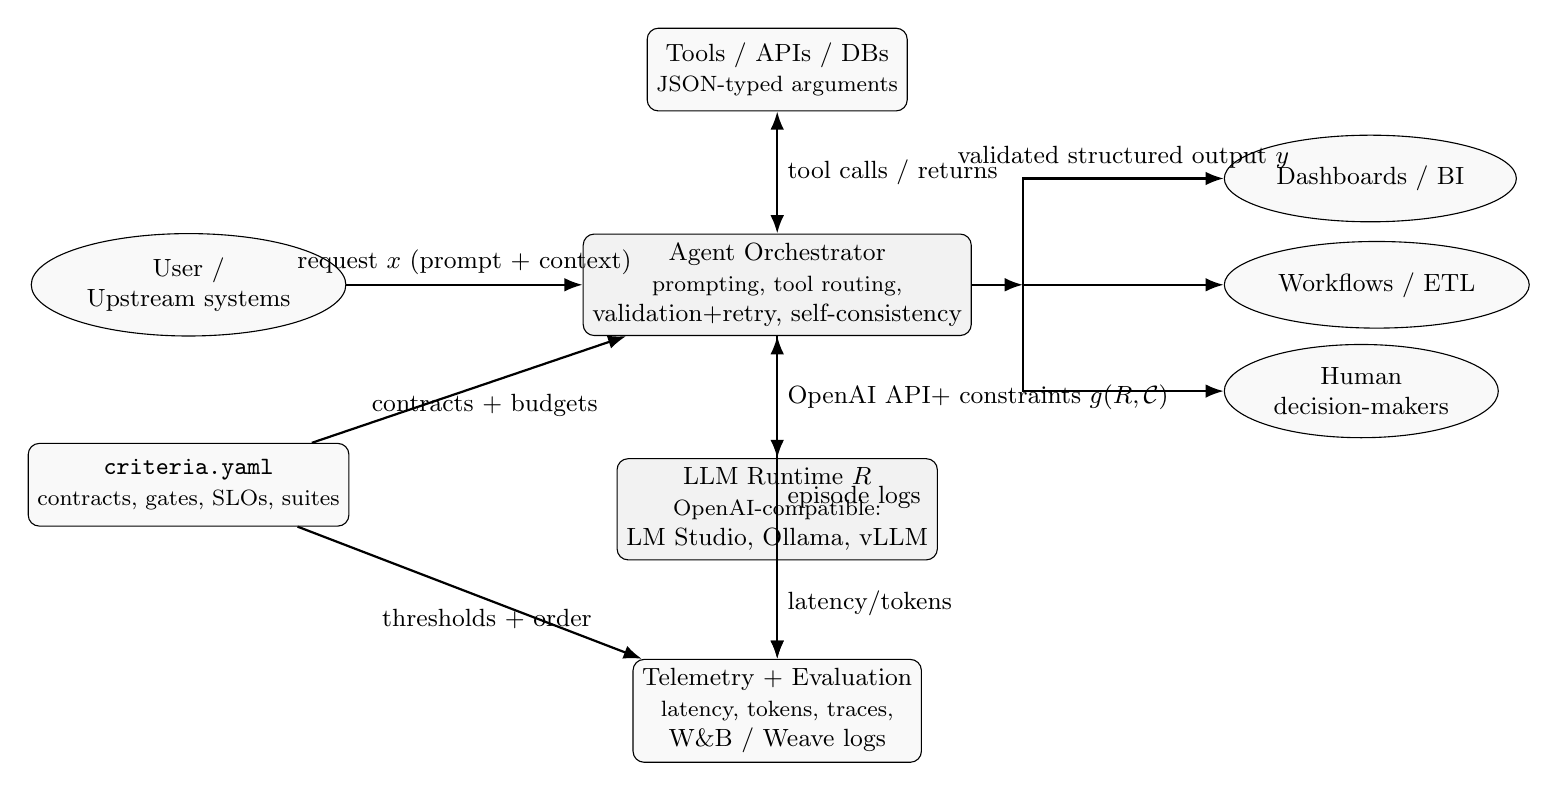
\begin{tikzpicture}[
    font=\small,
    node distance=1.55cm and 2.6cm,
    ext/.style={draw, ellipse, align=center, minimum width=2.9cm, minimum height=1.1cm, fill=gray!5},
    box/.style={draw, rounded corners, align=center, minimum width=3.6cm, minimum height=1.2cm, fill=gray!10},
    sbox/.style={draw, rounded corners, align=center, minimum width=3.1cm, minimum height=1.05cm, fill=gray!5},
    line/.style={-Latex, thick},
    bidir/.style={Latex-Latex, thick}
]

% Core nodes
\node[ext] (up) {User /\\ Upstream systems};
\node[box, right=3.0cm of up] (agent) {Agent Orchestrator\\ \footnotesize prompting, tool routing,\\ validation+retry, self-consistency};
\node[box, below=1.55cm of agent] (runtime) {LLM Runtime $R$\\ \footnotesize OpenAI-compatible:\\ LM Studio, Ollama, vLLM};
\node[sbox, above=1.55cm of agent] (tools) {Tools / APIs / DBs\\ \footnotesize JSON-typed arguments};
\node[sbox, below=1.35cm of up] (criteria) {\texttt{criteria.yaml}\\ \footnotesize contracts, gates, SLOs, suites};
\node[sbox, below=1.25cm of runtime] (obs) {Telemetry + Evaluation\\ \footnotesize latency, tokens, traces,\\ W\&B / Weave logs};

% Downstream consumers (right side)
\node[ext, right=3.2cm of agent, yshift=1.35cm] (dash) {Dashboards / BI};
\node[ext, right=3.2cm of agent] (etl) {Workflows / ETL};
\node[ext, right=3.2cm of agent, yshift=-1.35cm] (hum) {Human\\ decision-makers};

% Arrows
\draw[line] (up) -- node[above]{request $x$ (prompt + context)} (agent);

\draw[bidir] (agent) -- node[right]{OpenAI API\\ + constraints $g(R,\mathcal{C})$} (runtime);

\draw[bidir] (agent) -- node[right]{tool calls / returns} (tools);

\draw[line] (criteria) -- node[below,pos=0.55]{thresholds + order} (obs);
\draw[line] (criteria) -- node[below,pos=0.55]{contracts + budgets} (agent);

\draw[line] (agent.south) -- node[right]{episode logs} (obs.north);
\draw[line] (runtime.south) -- ++(0,-0.55) -| node[pos=0.25,right]{latency/tokens} (obs.north);

\draw[line] (agent.east) -- ++(0.65,0) coordinate (out);
\draw[line] (out) |- node[above,pos=0.75]{validated structured output $y$} (dash.west);
\draw[line] (out) |- (etl.west);
\draw[line] (out) |- (hum.west);

\end{tikzpicture}
\caption{System context for a contract-first, single-node agent.
An orchestrator mediates between upstream requests and downstream consumers, calling an OpenAI-compatible runtime and external tools, while enforcing contracts via backend constraints and validation.
Telemetry and evaluation log structure/accuracy/faithfulness/tool/stability/SLO metrics under a single versioned policy surface (\texttt{criteria.yaml}).}
\label{fig:agent-context}
\end{figure}

\begin{figure}[t]
\centering
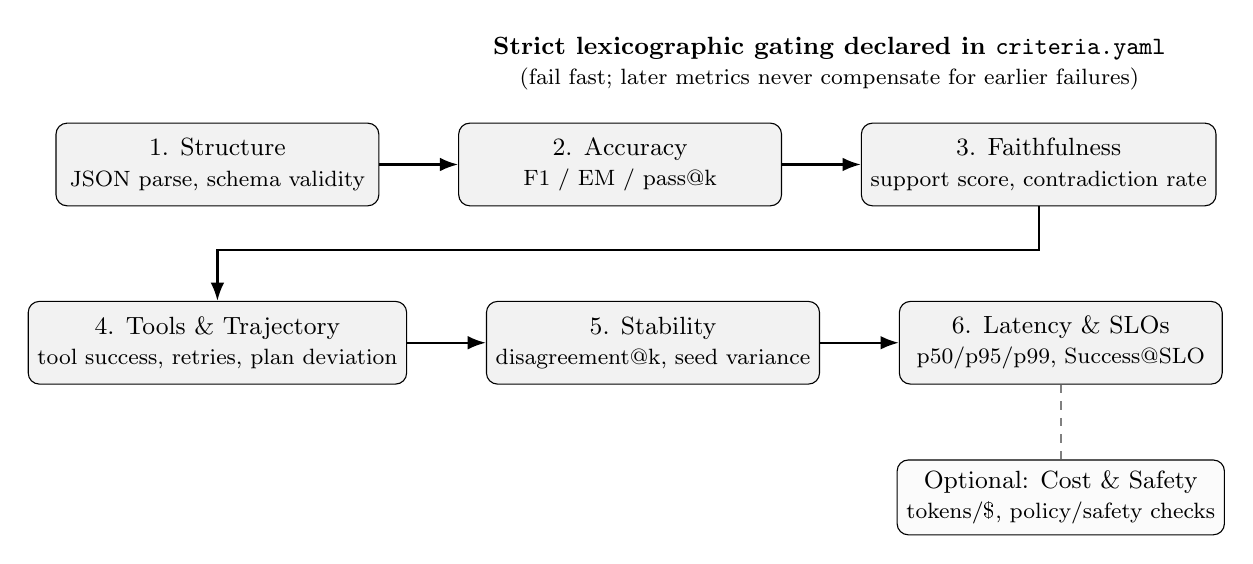
\begin{tikzpicture}[
    font=\small,
    node distance=0.9cm and 1.0cm,
    fam/.style={draw, rounded corners, align=center, minimum width=4.1cm, minimum height=1.05cm, fill=gray!10},
    opt/.style={draw, rounded corners, align=center, minimum width=4.1cm, minimum height=0.95cm, fill=gray!3},
    line/.style={-Latex, thick}
]

\node[fam] (s1) {1. Structure\\ \footnotesize JSON parse, schema validity};
\node[fam, right=1.0cm of s1] (s2) {2. Accuracy\\ \footnotesize F1 / EM / pass@k};
\node[fam, right=1.0cm of s2] (s3) {3. Faithfulness\\ \footnotesize support score, contradiction rate};

\node[fam, below=1.2cm of s1] (s4) {4. Tools \& Trajectory\\ \footnotesize tool success, retries, plan deviation};
\node[fam, right=1.0cm of s4] (s5) {5. Stability\\ \footnotesize disagreement@k, seed variance};
\node[fam, right=1.0cm of s5] (s6) {6. Latency \& SLOs\\ \footnotesize p50/\pninetyfive/\pninetynine, Success@\slo};

% Gating arrows (strict order)
\draw[line] (s1) -- (s2);
\draw[line] (s2) -- (s3);
\draw[line] (s3.south) -- ++(0,-0.55) -| (s4.north);
\draw[line] (s4) -- (s5);
\draw[line] (s5) -- (s6);

\node[opt, below=0.95cm of s6] (s7) {Optional: Cost \& Safety\\ \footnotesize tokens/\$, policy/safety checks};

\draw[dashed, gray, thick] (s6.south) -- (s7.north);

\node[align=center] at ($(s2.north)!0.5!(s3.north)+(0,0.75)$)
{\textbf{Strict lexicographic gating declared in \texttt{criteria.yaml}}\\
\footnotesize (fail fast; later metrics never compensate for earlier failures)};

\end{tikzpicture}
\caption{Metric families and strict gating order.
We evaluate structure, accuracy, and faithfulness before considering tools/trajectory, stability, and finally SLO adherence.
This ordering reflects production preference: a faster agent does not compensate for broken contracts or unfaithful outputs.}
\label{fig:metric-families}
\end{figure}

\begin{figure}[t]
\centering
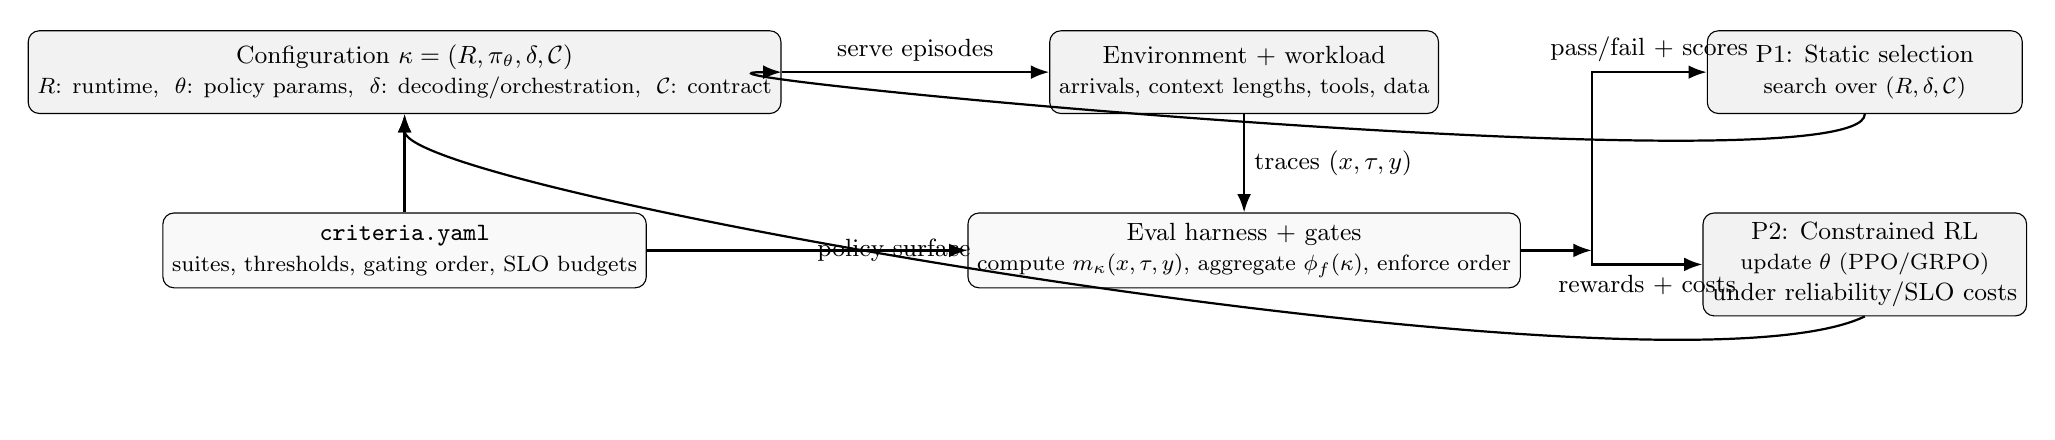
\begin{tikzpicture}[
    font=\small,
    node distance=1.4cm and 2.2cm,
    box/.style={draw, rounded corners, align=center, minimum width=4.0cm, minimum height=1.05cm, fill=gray!10},
    sbox/.style={draw, rounded corners, align=center, minimum width=3.2cm, minimum height=0.95cm, fill=gray!5},
    line/.style={-Latex, thick}
]

\node[box] (config) {Configuration $\kappa=(R,\pi_\theta,\delta,\mathcal{C})$\\
\footnotesize $R$: runtime,\ \ $\theta$: policy params,\ \ $\delta$: decoding/orchestration,\ \ $\mathcal{C}$: contract};

\node[box, right=3.4cm of config] (env) {Environment + workload\\ \footnotesize arrivals, context lengths, tools, data};

\node[sbox, below=1.25cm of env] (eval) {Eval harness + gates\\ \footnotesize compute $m_\kappa(x,\tau,y)$,\ aggregate $\phi_f(\kappa)$,\ enforce order};

\node[sbox, below=1.25cm of config] (crit) {\texttt{criteria.yaml}\\ \footnotesize suites, thresholds, gating order, SLO budgets};

\node[box, right=3.4cm of env] (search) {P1: Static selection\\ \footnotesize search over $(R,\delta,\mathcal{C})$};

\node[box, below=1.25cm of search] (rl) {P2: Constrained RL\\ \footnotesize update $\theta$ (PPO/GRPO)\\ under reliability/SLO costs};

% Forward path
\draw[line] (config) -- node[above]{serve episodes} (env);
\draw[line] (env) -- node[right]{traces $(x,\tau,y)$} (eval);

% Criteria into eval
\draw[line] (crit) -- node[right]{policy surface} (eval);
\draw[line] (crit.north) -- ++(0,0.35) -| (config.south);

% Metrics to selection and RL
\draw[line] (eval.east) -- ++(0.9,0) coordinate (mid);
\draw[line] (mid) |- node[above,pos=0.75]{pass/fail + scores} (search.west);
\draw[line] (mid) |- node[below,pos=0.75]{rewards + costs} (rl.west);

% Feedback
\draw[line] (search.south) .. controls +(0,-1.0) and +(-2.2,0.0) .. (config.east);
\draw[line] (rl.south) .. controls +(-2.5,-1.2) and +(0,-1.0) .. (config.south);

\end{tikzpicture}
\caption{Optimization view.
A configuration induces episodes under a workload/environment, which are scored by an eval harness governed by \texttt{criteria.yaml}.
P1 selects configurations by searching over runtimes and decoding/orchestration settings; P2 improves the policy parameters $\theta$ under explicit reliability and SLO constraints.}
\label{fig:optimization-view}
\end{figure}


\section{Evaluation Framework and Test Families}
\label{sec:eval-framework}

Figure~\ref{fig:metric-families} summarized the metric families we track.
This section describes how SpecSLOEval turns those abstract families into concrete, repeatable tests that can be executed unchanged across single-GPU, OpenAI-compatible backends (LM Studio, Ollama, vLLM, \texttt{llama.cpp} wrappers).
Our goal is operational: produce evaluation artifacts that are (i) contract-first, (ii) SLO-aware (tail latency, not just averages), and (iii) auditable end-to-end so every aggregate number can be traced back to per-episode inputs/outputs, schema validations, tool transcripts, and (when used) judge-model decisions.

\paragraph{Design principles.}
SpecSLOEval is built around four principles that matter in production settings:

\begin{itemize}[leftmargin=12pt]
    \item \textbf{Contract-first by construction.} Every task declares an explicit output schema (JSON Schema or a backend-compatible equivalent). Structural validity is a first-order metric, not a best-effort prompt instruction.
    \item \textbf{Lexicographic gating.} We treat correctness/faithfulness as \emph{gates} and latency primarily as a \emph{constraint}. A configuration that is fast but structurally invalid or unfaithful is rejected.
    \item \textbf{Backend-agnostic measurement.} The harness assumes only an OpenAI-compatible API plus observability hooks (token counts and latency). Everything else is done by the harness: schema validation, error taxonomies, tool mocks, stability repeats, and aggregation.
    \item \textbf{Auditability and reproducibility.} We log per-episode artifacts (inputs, outputs, parsed JSON, validation errors, tool traces, judge prompts/outputs) and experiment metadata (model, runtime, decoding params, schema version, git commit, seeds) to W\&B and optionally Weave (\url{https://docs.wandb.ai/models/quickstart}, \url{https://docs.wandb.ai/models/evaluate-models}).
\end{itemize}

\begin{figure}[t]
\centering
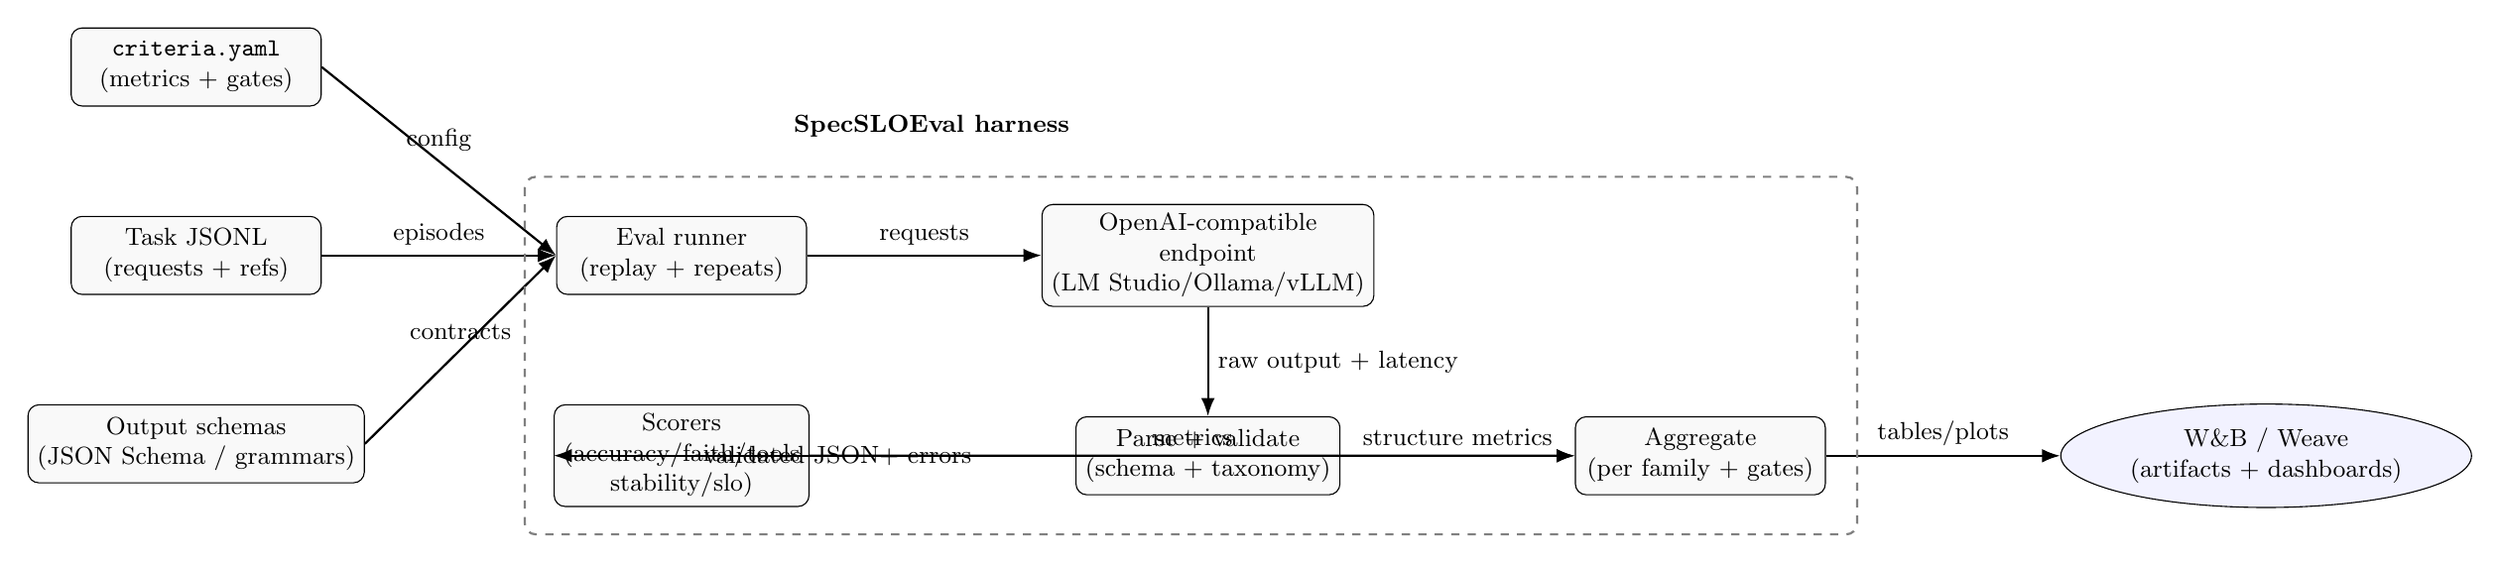
\begin{tikzpicture}[
    font=\small,
    node distance=1.4cm and 2.0cm,
    box/.style={draw, rounded corners, align=center, minimum width=3.2cm, minimum height=1.0cm, fill=gray!5},
    cloud/.style={draw, ellipse, align=center, minimum width=3.0cm, minimum height=1.0cm, fill=blue!5},
    line/.style={-Latex, thick}
]
    % Inputs
    \node[box] (criteria) {\texttt{criteria.yaml}\\(metrics + gates)};
    \node[box, below=of criteria] (tasks) {Task JSONL\\(requests + refs)};
    \node[box, below=of tasks] (schemas) {Output schemas\\(JSON Schema / grammars)};

    % Harness
    \node[box, right=3.0cm of tasks] (runner) {Eval runner\\(replay + repeats)};
    \node[box, right=3.0cm of runner] (backend) {OpenAI-compatible\\endpoint\\(LM Studio/Ollama/vLLM)};
    \node[box, below=of backend] (validate) {Parse + validate\\(schema + taxonomy)};
    \node[box, below=of runner] (scorers) {Scorers\\(accuracy/faith/tools\\stability/slo)};
    \node[box, right=3.0cm of validate] (agg) {Aggregate\\(per family + gates)};
    \node[cloud, right=3.0cm of agg] (wandb) {W\&B / Weave\\(artifacts + dashboards)};

    % Arrows
    \draw[line] (criteria.east) -- node[above]{config} (runner.west);
    \draw[line] (tasks.east) -- node[above]{episodes} (runner.west);
    \draw[line] (schemas.east) -- node[above]{contracts} (runner.west);

    \draw[line] (runner.east) -- node[above]{requests} (backend.west);
    \draw[line] (backend.south) -- node[right]{raw output + latency} (validate.north);
    \draw[line] (validate.west) -- ++(-1.2,0) |- node[left,pos=0.25]{validated JSON\\+ errors} (scorers.west);
    \draw[line] (scorers.east) -- node[above]{metrics} (agg.west);
    \draw[line] (validate.east) -- node[above]{structure metrics} (agg.west);

    \draw[line] (agg.east) -- node[above]{tables/plots} (wandb.west);

    % Dashed boundary around harness components
    \draw[rounded corners, thick, dashed, gray]
      ($(runner.north west)+(-0.4,0.5)$) rectangle
      ($(agg.south east)+(0.4,-0.5)$);

    \node[align=center, font=\small\bfseries] at ($(runner.north)+(3.2,1.15)$) {SpecSLOEval harness};

\end{tikzpicture}
\caption{SpecSLOEval evaluation architecture.
A single \texttt{criteria.yaml} and versioned task/schema artifacts drive an evaluation runner that replays episodes against an OpenAI-compatible backend.
The harness performs parsing/validation, computes per-family metrics (including stability repeats and SLO metrics), applies lexicographic gates, and logs all per-episode artifacts and aggregates to W\&B/Weave for auditability and reproducibility.}
\label{fig:eval-arch}
\end{figure}

\subsection{Evaluation Configuration via \texttt{criteria.yaml}}
\label{sec:criteria-yaml}

The entire framework is driven by a single configuration file, \texttt{agent\_eval/criteria.yaml}.
This file is the \emph{policy} of evaluation: it declares what to measure, what thresholds must hold, and how to aggregate across tasks and metric families.
Versioning this file alongside code is non-negotiable for trustworthy comparisons: when thresholds or gates change, the change is explicit and reviewable.

\paragraph{Schema surface.}
In our baseline design, \texttt{criteria.yaml} provides:

\begin{enumerate}[leftmargin=12pt]
    \item \textbf{Suites and task bindings:} a suite is a named grouping of tasks, where each task references a JSONL file and an output schema.
    \item \textbf{Gating policy:} an explicit order over metric families (e.g., structure $\rightarrow$ accuracy $\rightarrow$ faithfulness $\rightarrow$ tools $\rightarrow$ stability $\rightarrow$ SLO) and a policy (\texttt{strict} means earlier failures block later credit).
    \item \textbf{Thresholds:} per-metric pass thresholds or max violation rates (e.g., schema-validity $\ge 0.99$, contradiction rate $\le 0.05$).
    \item \textbf{SLO budgets:} p95/p99 targets, hard timeouts, and max tokens-out.
\end{enumerate}

\paragraph{Concrete example (aligned with our P1 suite).}
For clarity we show a simplified excerpt that matches the structure of the P1 criteria used in our runs (full file is versioned with the harness):

\begin{lstlisting}[basicstyle=\ttfamily\small]
schema_version: "1.0"
criteria_id: "p1_core_v1"

suites:
  p1_core:
    tasks:
      - id: "t1_clinc"
        family: "accuracy"
        task_file: "tasks/clinc_en.jsonl"
        output_schema: "tasks/schemas/clinc_nlu_schema.json"
      - id: "t2_hotpot"
        family: "faithfulness"
        task_file: "tasks/hotpot_dev.jsonl"
        output_schema: "tasks/schemas/hotpot_explainer_schema.json"
      - id: "t3_tools"
        family: "tools"
        task_file: "tasks/t3_tools.jsonl"
        output_schema: "tasks/schemas/t3_tool_call_schema.json"

gating:
  order: ["structure", "accuracy", "faithfulness", "tools", "stability", "slo"]
  policy: "strict"

structure:
  json_valid: 0.99

accuracy:
  clinc_intent_f1: 0.85
  hotpot_answer_em: 0.65

faithfulness:
  hotpot_faithfulness: 0.80
  hotpot_contradiction_rate_max: 0.05

tools:
  tool_success_rate: 0.90

stability:
  disagreement_max: 0.10

slo:
  success_at_slo: 0.75
  p95_ms: 1200
  p99_ms: 2000
  max_tokens_out: 512
\end{lstlisting}

\paragraph{Lexicographic gating (why it matters).}
Most teams implicitly behave lexicographically (``don’t ship broken JSON'' $\rightarrow$ ``don’t ship hallucinations'' $\rightarrow$ ``make it fast enough''), but many evaluation setups do not encode it.
We encode it explicitly so that automated comparisons reflect the real risk surface.

\begin{figure}[t]
\centering
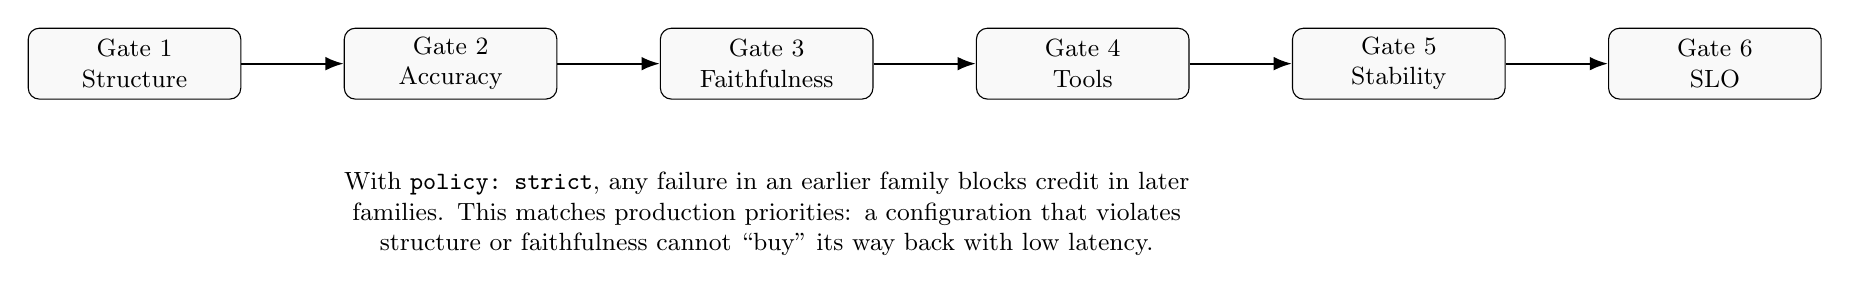
\begin{tikzpicture}[
    font=\small,
    node distance=0.9cm and 1.3cm,
    gate/.style={draw, rounded corners, align=center, minimum width=2.7cm, minimum height=0.9cm, fill=gray!5},
    line/.style={-Latex, thick}
]
    \node[gate] (g1) {Gate 1\\Structure};
    \node[gate, right=of g1] (g2) {Gate 2\\Accuracy};
    \node[gate, right=of g2] (g3) {Gate 3\\Faithfulness};
    \node[gate, right=of g3] (g4) {Gate 4\\Tools};
    \node[gate, right=of g4] (g5) {Gate 5\\Stability};
    \node[gate, right=of g5] (g6) {Gate 6\\SLO};

    \draw[line] (g1) -- (g2);
    \draw[line] (g2) -- (g3);
    \draw[line] (g3) -- (g4);
    \draw[line] (g4) -- (g5);
    \draw[line] (g5) -- (g6);

    \node[align=center, below=0.8cm of g3, text width=0.9\linewidth] (note)
    {With \texttt{policy: strict}, any failure in an earlier family blocks credit in later families.
     This matches production priorities: a configuration that violates structure or faithfulness cannot ``buy'' its way back with low latency.};

\end{tikzpicture}
\caption{Lexicographic gating in SpecSLOEval.
Evaluation proceeds in an explicit family order.
With strict gating, later families (e.g., SLO compliance) are considered only after earlier quality gates pass.}
\label{fig:criteria-gating}
\end{figure}

\subsection{Per-Episode Record and Audit Trail}
\label{sec:episode-record}

SpecSLOEval evaluates \emph{episodes}. Each episode produces a structured record (stored as JSON and logged as an artifact) containing:

\begin{itemize}[leftmargin=12pt]
    \item \textbf{Inputs:} request text, retrieved/context bundle, tool catalog snapshot, schema identifiers.
    \item \textbf{Outputs:} raw model output, parsed JSON (if parse succeeds), tool call transcript.
    \item \textbf{Observability:} latency (end-to-end and TTFT when available), token counts, retries, backend identifiers, decoding params, random seeds.
    \item \textbf{Evaluations:} structure validity flags and error taxonomy; task accuracy components; faithfulness judge artifacts (prompts, extracted claims, support scores, contradiction flags); stability repeats linkage; SLO success flags.
\end{itemize}

This record is what makes the framework \emph{publishable}: tables and plots can be reproduced by re-aggregating immutable episode artifacts under a fixed criteria version.

\subsection{Test Families}
\label{sec:test-families}

We group tests into six families: \emph{Structure}, \emph{Task Accuracy}, \emph{Faithfulness}, \emph{Tools/Trajectory}, \emph{Stability}, and \emph{Latency/SLO}.
Each family maps cleanly to real operational risks, which is why we treat them as first-class objects in \texttt{criteria.yaml} rather than ad-hoc metrics.

\begin{table}[t]
\centering
\small
\begin{tabular}{@{}p{2.4cm}p{5.3cm}p{5.2cm}@{}}
\toprule
\textbf{Family} & \textbf{What it measures} & \textbf{Typical failures caught} \\
\midrule
Structure & JSON parse + schema validity + error taxonomy & malformed JSON, missing/extra fields, type mismatches, invalid enums \\
Accuracy & label correctness (F1/EM/acc/pass@k) & wrong intent/answer, inconsistent field extraction \\
Faithfulness & support of claims against context (judge + atomic facts) & hallucinated statements, numeric sign errors, contradictions \\
Tools/Trajectory & tool-call validity, success, plan quality, redundancy & invalid tool args, tool thrashing, redundant calls, wrong sequencing \\
Stability & disagreement across repeats/seeds under fixed config & nondeterministic outputs, brittle prompts/decoding, unstable scores \\
Latency/SLO & p50/p95/p99 latency, Success@\slo, violation rates & tail-latency collapse, timeouts, throughput collapse under load \\
\bottomrule
\end{tabular}
\caption{Metric families and the operational risks they are designed to detect.
SpecSLOEval evaluates agents as services: structure and faithfulness failures are treated as deployment blockers; latency is treated primarily as a constraint.}
\label{tab:families}
\end{table}

\subsubsection{Structure: JSON and Schema Correctness}

The structure family measures whether outputs can be consumed by downstream systems without bespoke cleanup.
We compute two primary indicators per episode:
(i) JSON parse success; and (ii) schema validity under the declared contract $\mathcal{C}$.
We additionally record a fine-grained error taxonomy (e.g., missing required fields, additional properties, type mismatches, constraint violations), because aggregate validity alone is insufficient for debugging.

\paragraph{Parameters.}
Each structural test is defined by:
\begin{itemize}[leftmargin=12pt]
    \item a schema/contract $\mathcal{C}$ (name + version),
    \item prompts/tasks that exercise the schema (including adversarial formatting cases),
    \item pass thresholds such as \texttt{json\_valid} $\ge 0.99$.
\end{itemize}

\paragraph{Example S1: Basic JSON/Schema Validity.}
Fix a moderate schema $\mathcal{C}_{\text{basic}}$ (nested objects, bounded arrays).
Run on $N$ prompts and compute
\[
m_{\text{json}} = \frac{\#\text{episodes with parse \& schema valid}}{N}.
\]
We gate with $m_{\text{json}} \ge 0.99$ for the P1 suite because rare structural failures are operationally catastrophic.

\paragraph{Example S2: Schema Evolution Robustness.}
Given $(\mathcal{C}_1,\mathcal{C}_2)$ where $\mathcal{C}_2$ adds optional fields or relaxes bounds, we test:
(i) regression in validity when switching schemas; and (ii) whether the agent can emit outputs valid under both (when that is a requirement for rolling upgrades).

\subsubsection{Task Accuracy: F1, EM, and pass@\texorpdfstring{$k$}{k}}

The accuracy family measures task correctness against references.
We intentionally keep accuracy metrics \emph{separate} from structure metrics: a run can be structurally perfect and still wrong.

\paragraph{Parameters.}
Accuracy tests specify:
\begin{itemize}[leftmargin=12pt]
    \item a dataset $\mathcal{D}_{\text{acc}} = \{(x_i, y_i^{\text{ref}})\}$,
    \item a schema $\mathcal{C}$ for predictions,
    \item a scoring map from predicted JSON fields to labels/answers,
    \item pass thresholds (e.g., intent F1 $\ge 0.85$, QA EM $\ge 0.65$).
\end{itemize}

\paragraph{Example A1: Field-Level Extraction F1.}
For extraction/classification tasks we compute macro-F1 across the evaluated JSON fields.
This directly measures whether the agent can reliably populate structured fields, not merely produce valid JSON.

\paragraph{Example A2: Programmatic QA Exact Match and pass@\,$k$.}
For QA-style tasks we embed the answer in a simple schema (e.g., \texttt{final\_answer}) and compute EM/F1.
When sampling is enabled, pass@\,$k$ measures whether any of $k$ samples matches the reference.

\subsubsection{Faithfulness: LLM-as-Judge with Atomic Statements}

Faithfulness measures whether the agent’s statements are supported by the provided context $C$.
We operationalize this using an LLM-as-judge pipeline inspired by RAGAS~\citep{es2023ragas} and atomic-fact approaches~\citep{atomicFacts2024}, but with explicit structure:

\begin{enumerate}[leftmargin=12pt]
    \item Extract \emph{atomic statements} from the agent output (restricted to designated fields, e.g., a narrative explanation field).
    \item For each statement, ask a judge to score support on a 0--3 scale and flag contradictions.
    \item Aggregate into a normalized faithfulness score and a contradiction rate, both used for gating.
\end{enumerate}

\begin{figure}[t]
\centering
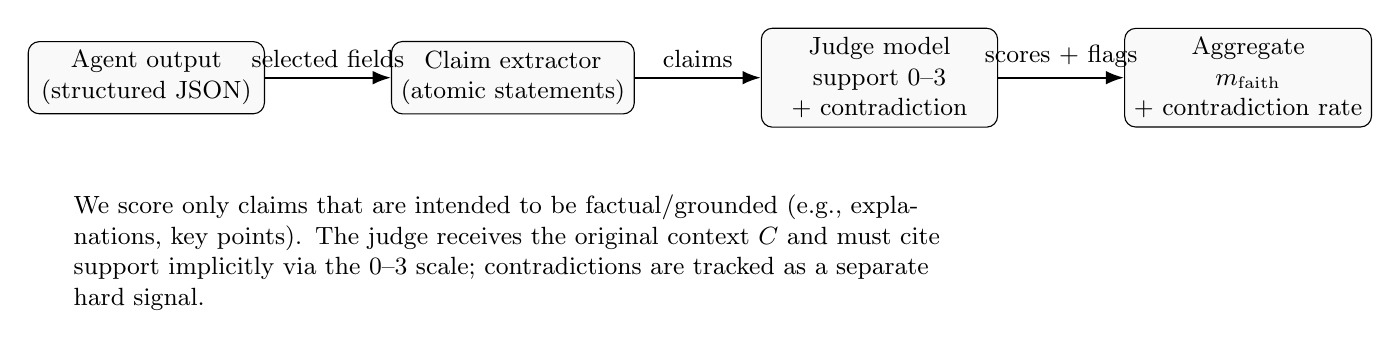
\begin{tikzpicture}[
    font=\small,
    node distance=1.2cm and 1.6cm,
    box/.style={draw, rounded corners, align=center, minimum width=3.0cm, minimum height=0.9cm, fill=gray!5},
    line/.style={-Latex, thick}
]
    \node[box] (out) {Agent output\\(structured JSON)};
    \node[box, right=of out] (extract) {Claim extractor\\(atomic statements)};
    \node[box, right=of extract] (judge) {Judge model\\support 0--3\\+ contradiction};
    \node[box, right=of judge] (agg) {Aggregate\\$m_{\text{faith}}$\\+ contradiction rate};

    \draw[line] (out) -- node[above]{selected fields} (extract);
    \draw[line] (extract) -- node[above]{claims} (judge);
    \draw[line] (judge) -- node[above]{scores + flags} (agg);

    \node[align=left, below=0.9cm of extract, text width=0.92\linewidth]
    {We score only claims that are intended to be factual/grounded (e.g., explanations, key points).
     The judge receives the original context $C$ and must cite support implicitly via the 0--3 scale; contradictions are tracked as a separate hard signal.};

\end{tikzpicture}
\caption{Faithfulness evaluation pipeline in SpecSLOEval.
We decompose outputs into atomic statements and score each against context using a judge model.
The aggregate faithfulness score and contradiction rate are used for gating and are logged with full judge prompts/outputs for auditing.}
\label{fig:faithfulness-pipeline}
\end{figure}

\paragraph{Scoring.}
Let $S$ be the set of extracted statements and $s_j \in \{0,1,2,3\}$ the judge support score for statement $j$ with contradiction flag $c_j \in \{0,1\}$.
We define an aggregate (one reasonable instantiation) as:
\[
m_{\text{faith}}(x,y) =
\max\left(0,\;
\frac{1}{|S|}\sum_{j \in S}\frac{s_j}{3}
\;-\;
\lambda_{\text{contr}}\cdot\frac{1}{|S|}\sum_{j \in S} c_j
\right),
\]
with $\lambda_{\text{contr}}$ set so that even a small contradiction rate meaningfully depresses the score.
We also gate on a maximum contradiction rate (e.g., $\le 0.05$) because contradictions are qualitatively worse than omissions.

\paragraph{Example F1: Grounded Narrative Summaries.}
The agent writes a short summary and key points from retrieved documents.
The judge decomposes these into claims and scores them.
We require $m_{\text{faith}} \ge 0.75$ and contradiction rate $\le 5\%$ on the P1 grounded QA suite.

\paragraph{Example F2: Numeric and Trend Consistency.}
When contexts include metrics/time-series, we explicitly prompt the judge to focus on directionality and magnitude.
This catches the most damaging real-world hallucinations in analytics/monitoring agents: sign inversions, fabricated deltas, and exaggerated trends.

\subsubsection{Tools and Trajectories}

For tool-using agents, final output quality is insufficient: operational reliability depends on whether tool calls are valid, succeed, and are not wasteful.
We evaluate both \emph{tool-call validity} (arguments satisfy the tool schema) and \emph{trajectory quality} (no thrashing, minimal redundancy, appropriate sequencing).

\begin{figure}[t]
\centering
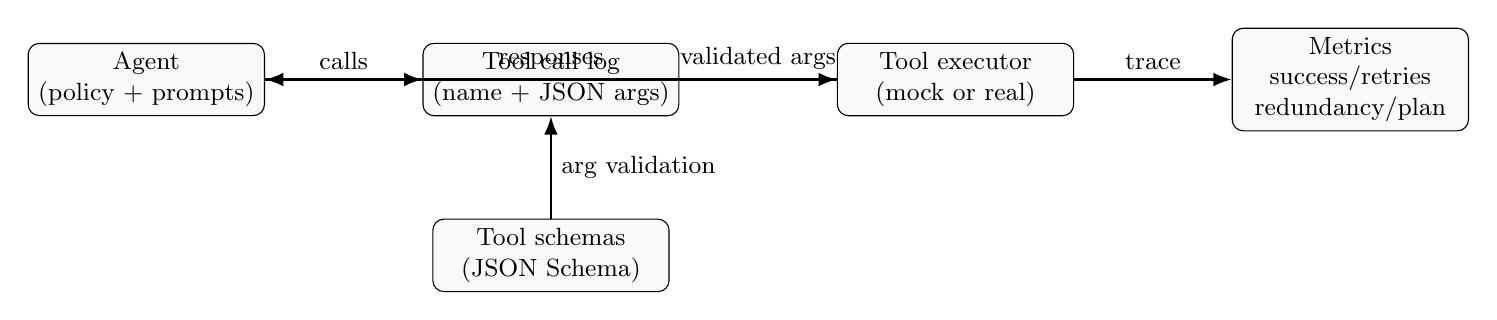
\begin{tikzpicture}[
    font=\small,
    node distance=1.3cm and 2.0cm,
    box/.style={draw, rounded corners, align=center, minimum width=3.0cm, minimum height=0.9cm, fill=gray!5},
    line/.style={-Latex, thick}
]
    \node[box] (agent) {Agent\\(policy + prompts)};
    \node[box, right=of agent] (calls) {Tool call log\\(name + JSON args)};
    \node[box, right=of calls] (mock) {Tool executor\\(mock or real)};
    \node[box, below=of calls] (schemas) {Tool schemas\\(JSON Schema)};
    \node[box, right=of mock] (metrics) {Metrics\\success/retries\\redundancy/plan};

    \draw[line] (agent) -- node[above]{calls} (calls);
    \draw[line] (calls) -- node[above]{validated args} (mock);
    \draw[line] (schemas) -- node[right]{arg validation} (calls.south);
    \draw[line] (mock) -- node[above]{responses} (agent.east);
    \draw[line] (mock) -- node[above]{trace} (metrics);

\end{tikzpicture}
\caption{Tool and trajectory evaluation.
We validate tool arguments against declared schemas, execute tools (mocked deterministically for reproducibility or real services when available), and compute tool success and trajectory efficiency metrics from the full trace.}
\label{fig:tools-traj}
\end{figure}

\paragraph{Parameters.}
Tool tests specify:
\begin{itemize}[leftmargin=12pt]
    \item a tool catalog (tool names, descriptions, JSON argument schemas),
    \item an executor (deterministic mock for CI; optionally real services in staging),
    \item optional canonical plans (minimal tool sequences),
    \item thresholds (e.g., tool success $\ge 0.90$; redundant calls bounded).
\end{itemize}

\paragraph{Example T1: Tool-Argument Validity and Success Rate.}
We validate each tool call against its argument schema; the executor returns success/failure deterministically.
We compute
\[
m_{\text{tool}} = \frac{\#\text{successful tool calls}}{\#\text{tool calls}},
\]
and gate on $m_{\text{tool}} \ge 0.90$.

\paragraph{Example T2: Trajectory Cost, Redundancy, and Plan Deviation.}
When a canonical plan exists, we compute edit distance between observed and expected tool sequences, plus counts of extra calls and invalid retries.
These metrics are operationally important because tool thrashing inflates tail latency and can trip downstream rate limits.

\subsubsection{Stability Across Runs}

Stability is the most under-measured production risk: unstable structured outputs break monitoring, A/B comparisons, and trust.
We define stability tests by repeating identical episodes under fixed configuration and measuring output disagreement.

\paragraph{Parameters.}
Stability tests specify:
\begin{itemize}[leftmargin=12pt]
    \item a prompt set $\mathcal{D}_{\text{stab}}$ representative of the workload,
    \item a number of repeats $k$ per input (e.g., $k=5$ or $k=20$),
    \item an equivalence rule: exact JSON equality, canonical JSON equality, or claim-overlap equivalence.
\end{itemize}

\paragraph{Example ST1: Disagreement@\,$k$ for Structured Outputs.}
Run $k$ times per input. Let $\mathrm{Eq}(y^{(a)},y^{(b)})$ be equivalence under canonicalization.
Define Disagreement@\,$k$ as
\[
\mathrm{Disagree}@k = 1 - \frac{\#\text{runs matching the modal output}}{k},
\]
and gate on \(\mathrm{Disagree}@k \le 0.10\) (as in our P1 criteria) for stability-sensitive deployments.

\paragraph{Example ST2: Seed Variance on Accuracy and Faithfulness.}
We evaluate across multiple seeds and compute variance in macro-F1 and faithfulness.
High variance indicates brittle behavior even if the mean score is acceptable.

\subsubsection{Latency and SLO Tests}

Latency/SLO tests measure whether configurations satisfy tail-latency commitments under realistic request mixes and (optionally) load.
We focus on p95 and p99 because these are the operational pain points in multi-step agent flows, consistent with “The Tail at Scale”~\citep{dean2013tail} and modern LLM serving work~\citep{kwon2023vllm,agrawal2024sarathi}.

\paragraph{Workloads.}
We parameterize workloads by:
\begin{itemize}[leftmargin=12pt]
    \item context length distribution (short vs long contexts),
    \item output token budgets,
    \item arrival process (steady Poisson; bursty sequences),
    \item tool-use frequency (for tool-heavy agent mixes).
\end{itemize}

\begin{figure}[t]
\centering
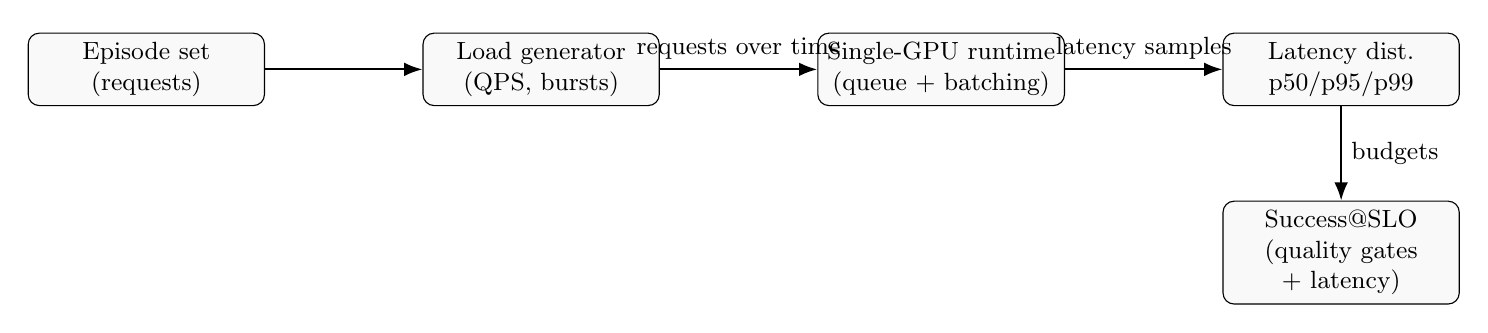
\begin{tikzpicture}[
    font=\small,
    node distance=1.2cm and 2.0cm,
    box/.style={draw, rounded corners, align=center, minimum width=3.0cm, minimum height=0.9cm, fill=gray!5},
    line/.style={-Latex, thick}
]
    \node[box] (dataset) {Episode set\\(requests)};
    \node[box, right=of dataset] (load) {Load generator\\(QPS, bursts)};
    \node[box, right=of load] (runtime) {Single-GPU runtime\\(queue + batching)};
    \node[box, right=of runtime] (dist) {Latency dist.\\p50/p95/p99};
    \node[box, below=of dist] (success) {Success@\slo\\(quality gates\\+ latency)};
    \draw[line] (dataset) -- (load);
    \draw[line] (load) -- node[above]{requests over time} (runtime);
    \draw[line] (runtime) -- node[above]{latency samples} (dist);
    \draw[line] (dist) -- node[right]{budgets} (success);
\end{tikzpicture}
\caption{Latency/SLO evaluation.
A workload generator replays an episode set under a specified arrival process to a single-GPU runtime.
We compute p50/p95/p99 latency and Success@\slo, where an episode counts only if it passes quality gates \emph{and} meets latency budgets.}
\label{fig:slo-eval}
\end{figure}

\paragraph{Example L1: Success@\slo under Mixed Load.}
For each episode we compute quality metrics (structure/accuracy/faithfulness/tools/stability where applicable) and latency $L_\kappa(x)$.
We then define Success@\slo as:
\[
\text{Success@\slo}_\kappa(x)=
\mathbf{1}\{\text{quality gates pass}\}\cdot \mathbf{1}\{L_\kappa(x)\le B\},
\]
and aggregate to get a business-aligned “good and on-time” rate.

\paragraph{Example L2: QPS vs p95 Curves and Configuration Frontier.}
We sweep QPS levels and plot QPS vs p95/p99 and QPS vs Success@\slo, producing an operating frontier for each configuration.
This makes tail collapse visible and supports principled choices of token budgets, batching, and self-consistency depth.

\subsection{Extensibility, Logging, and Use in RL}
\label{sec:extensibility-rl}

\paragraph{Extending the metric space.}
SpecSLOEval is intentionally modular.
Adding a metric means:
(i) adding a key and threshold in \texttt{criteria.yaml}; and
(ii) implementing a scorer function that consumes the per-episode record.
This supports domain metrics (e.g., “invoice total reconciles,” “campaign budget constraint satisfied”) without rewriting the harness.

\paragraph{Logging and auditability.}
All runs are logged to W\&B, including:
\begin{itemize}[leftmargin=12pt]
    \item per-episode artifacts (inputs, outputs, parsed JSON, error taxonomy, tool traces, judge artifacts),
    \item per-run configuration (backend, model id, decoding params, schema versions, criteria version),
    \item aggregated tables/plots (per-family metrics, gating pass/fail, latency quantiles, Success@\slo).
\end{itemize}
We optionally instrument judge pipelines and multi-stage scoring in Weave so that intermediate computations can be inspected and replayed.

\paragraph{Bridging evaluation and optimization (P2).}
The same metric vector that gates deployments also defines reward/cost surfaces for SLO-aware RL.
Concretely, we can define a scalar reward for an episode by combining metric components:
\[
r(x,y) = \sum_{k} w_k\, m_k(x,y) \;-\; \beta\,\max(0, L(x)-B),
\]
while treating contradiction rate, repeated schema failures, or SLO violations as explicit costs in constrained RL~\citep{altman1999cmdp,achiam2017cpo}.
This design minimizes the common failure mode where “training metrics” and “deployment metrics” diverge.

\medskip
In Section~\ref{sec:experiments} we instantiate these test families on single-GPU backends and demonstrate how spec-driven decoding and bounded retry/self-consistency shift the trade-off frontier between structural correctness, faithfulness, stability, and tail latency.

\section{Experiments}
\label{sec:experiments}

This section instantiates SpecSLOEval in a concrete, single-GPU setting and reports how decoding \emph{constraints} (schemas/grammars), \emph{guardrails} (validation-and-retry), and \emph{budgeted self-consistency} interact with the full metric vector from Figure~\ref{fig:metric-families}.
Our goals are to demonstrate that:
(i) contract-first agents can be served on commodity single-node stacks without sacrificing reliability;
(ii) structural correctness, task performance, faithfulness, tool behavior, stability, and tail latency can be measured \emph{together} under a single criteria contract; and
(iii) the resulting measurements cleanly support both static configuration selection (P1) and SLO-aware policy optimization (P2).

\paragraph{Section roadmap.}
Section~\ref{sec:setup} describes hardware, backends, models, and reproducibility practices.
Section~\ref{sec:tasks} defines the P1 core suite (CLINC intent, HotpotQA grounded QA, and tool calls) and the associated JSON contracts.
Section~\ref{sec:baselines-configs} specifies the compared configurations (U/P/P+V/G/S) and the knobs we hold fixed.
Section~\ref{sec:metrics-reporting} defines our reporting protocol (aggregation, confidence intervals, and SLO accounting).
Sections~\ref{sec:results-structure-faith}--\ref{sec:results-backends} summarize representative findings and the analyses enabled by the framework.

\begin{figure}[t]
\centering
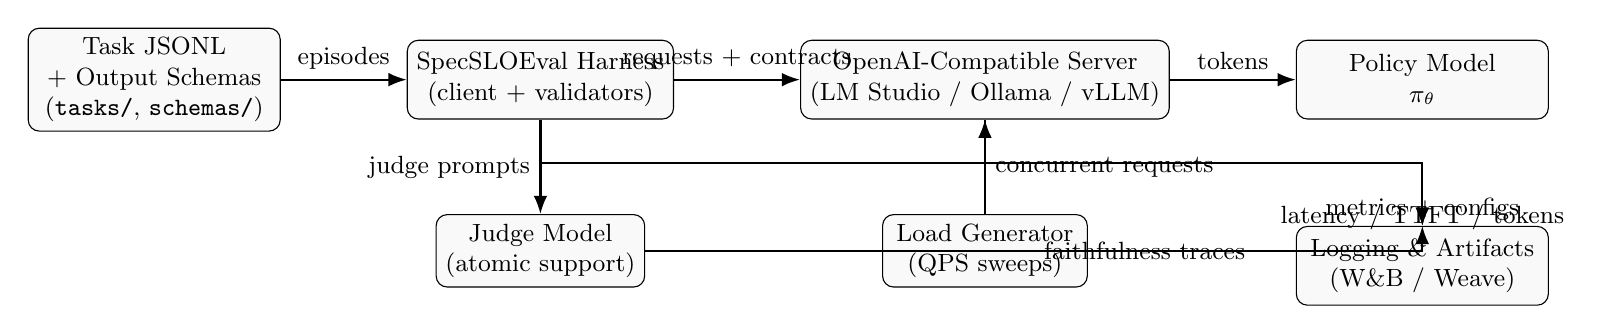
\begin{tikzpicture}[
    font=\small,
    node distance=1.2cm and 1.6cm,
    box/.style={draw, rounded corners, align=center, minimum width=3.2cm, minimum height=1.0cm, fill=gray!5},
    smallbox/.style={draw, rounded corners, align=center, minimum width=2.6cm, minimum height=0.9cm, fill=gray!5},
    line/.style={-Latex, thick}
]
\node[box] (tasks) {Task JSONL\\ + Output Schemas\\ (\texttt{tasks/}, \texttt{schemas/})};
\node[box, right=of tasks] (harness) {SpecSLOEval Harness\\ (client + validators)};
\node[box, right=of harness] (server) {OpenAI-Compatible Server\\ (LM Studio / Ollama / vLLM)};
\node[box, right=of server] (model) {Policy Model\\ $\pi_\theta$};

\node[smallbox, below=of harness] (judge) {Judge Model\\ (atomic support)};
\node[smallbox, below=of server] (load) {Load Generator\\ (QPS sweeps)};
\node[box, below=1.35cm of model] (wandb) {Logging \& Artifacts\\ (W\&B / Weave)};

\draw[line] (tasks) -- node[above]{episodes} (harness);
\draw[line] (harness) -- node[above]{requests + contracts} (server);
\draw[line] (server) -- node[above]{tokens} (model);

\draw[line] (harness.south) -- node[left]{judge prompts} (judge.north);
\draw[line] (judge.east) -| node[pos=0.25,right]{faithfulness traces} (wandb.north);

\draw[line] (load.north) -- node[right]{concurrent requests} (server.south);
\draw[line] (server.south) -- ++(0,-0.55) -| node[pos=0.75,below]{latency / TTFT / tokens} (wandb.north);

\draw[line] (harness.south) -- ++(0,-0.55) -| node[pos=0.7,below]{metrics + configs} (wandb.north);

\end{tikzpicture}
\caption{End-to-end experimental pipeline.
SpecSLOEval consumes task JSONL and JSON Schemas, executes episodes through an OpenAI-compatible server, validates outputs, optionally calls a judge model for faithfulness, and logs per-episode traces and aggregates to W\&B/Weave. Latency/SLO experiments add a load generator that drives QPS sweeps against the same endpoints.}
\label{fig:exp-pipeline}
\end{figure}

\subsection{Experimental Setup}
\label{sec:setup}

\paragraph{Hardware.}
Unless otherwise noted, experiments run on two representative single-node deployments:

\begin{itemize}[leftmargin=12pt]
    \item \textbf{RTX~4090 workstation:} NVIDIA RTX~4090 (24~GB VRAM), 64~GB system RAM, Ubuntu~22.04, CUDA~12.x with current NVIDIA drivers.
    \item \textbf{Apple Silicon laptop:} MacBook Pro with Apple M2 Max and 64~GB unified memory, macOS~15+.
\end{itemize}

\begin{table}[t]
\centering
\small
\begin{tabular}{@{}lcc@{}}
\toprule
\textbf{Component} & \textbf{4090 workstation} & \textbf{M2 Max laptop} \\
\midrule
Accelerator & RTX~4090 (24GB) & M2 Max (unified memory) \\
OS & Ubuntu~22.04 & macOS~15+ \\
Primary runtime & LM Studio server & LM Studio server \\
Alt. runtimes & Ollama, vLLM & Ollama (optional) \\
Primary usage & throughput / tail latency & portability / local dev \\
\bottomrule
\end{tabular}
\caption{Hardware/runtime matrix for the single-node regime targeted in this paper.}
\label{tab:hw-matrix}
\end{table}

\paragraph{Serving backends.}
All backends are exercised through an OpenAI-compatible HTTP interface.
Our primary runtime is LM Studio’s OpenAI-compatible server (\url{https://lmstudio.ai/docs/developer/openai-compat/tools}).
We additionally evaluate Ollama (\url{https://docs.ollama.com/capabilities/structured-outputs}) and a vLLM-backed server (\url{https://arxiv.org/abs/2309.06180}) to expose differences in batching, KV-cache behavior, and tail latency under load.
The spec compiler (Section~\ref{sec:spec-compiler}) emits backend-specific constraint artifacts (JSON Schema, tool specs, or grammars) while keeping the \emph{contract} constant.

\paragraph{Models.}
We focus on open-weight instruction-tuned models that are practical in the single-GPU regime, using Qwen family checkpoints served locally (e.g., Qwen2.5 7B/14B).
For every run we log:
(i) model identifier and revision;
(ii) quantization and precision mode (e.g., BF16 vs quantized);
(iii) maximum context length and maximum output tokens;
(iv) decoding parameters and constraint mode.

\paragraph{Reproducibility and measurement hygiene.}
For each configuration we:
(i) run a warmup phase (to stabilize KV-cache allocation and page behavior);
(ii) record per-request \emph{client-side} end-to-end latency, including retries and validation;
(iii) fix explicit random seeds where supported and log all seeds;
(iv) export run configs, schemas, and datasets as versioned artifacts in W\&B.
Latency distributions are reported over full runs (not averages) and summarized with p50/\pninetyfive/\pninetynine.

\subsection{Tasks and Datasets}
\label{sec:tasks}

Our P1 core suite (mirroring \texttt{criteria.yaml}) comprises three task families with explicit JSON contracts and auditable metrics.
All tasks are stored as JSONL with a stable schema and versioned as artifacts.

\begin{table}[t]
\centering
\small
\begin{tabular}{@{}llll@{}}
\toprule
\textbf{Task} & \textbf{ID} & \textbf{Contract / Output} & \textbf{Primary metrics} \\
\midrule
Intent classification (CLINC) & T1 & intent label JSON & intent F1, accuracy, JSON validity \\
Grounded QA (HotpotQA) & T2 & answer + explanation JSON & EM/F1, faithfulness, contradiction rate \\
Tool-use episodes & T3 & tool call schema + outputs & tool success, JSON validity, retries \\
\bottomrule
\end{tabular}
\caption{P1 core task suite used throughout the experiments, aligned with the \texttt{criteria.yaml} contract.}
\label{tab:task-suite}
\end{table}

\paragraph{T1: CLINC intent classification.}
Each episode maps an utterance to an intent label under a strict JSON contract (e.g., \texttt{\{"intent": "...", "confidence": ...\}} or an equivalent schema).
We compute intent accuracy and macro-F1, plus structure metrics (JSON validity, schema validity).
This task isolates \emph{structured classification correctness} under constraints.

\paragraph{T2: HotpotQA grounded question answering.}
Each episode provides a question and a context bundle (retrieved passages) and requires a structured output containing a short answer and a brief explanation.
We score answer EM/F1 and compute faithfulness using our judge-based atomic support procedure (Section~\ref{sec:eval-framework}), including a maximum contradiction-rate gate.
This task probes the interaction between structured outputs and \emph{semantic grounding}.

\paragraph{T3: Tool-use episodes.}
Episodes require the agent to emit tool calls (with JSON-typed arguments) and a final structured result.
Tool calls are validated against JSON Schemas; mock tools return deterministic responses to isolate model behavior from external nondeterminism.
We measure tool-call success, invalid-argument rates, redundant calls, and overall episode Success@\slo.

\subsection{Baselines and Configurations}
\label{sec:baselines-configs}

We compare five configurations that progressively add contract enforcement and reliability mechanisms.
All configurations share the same underlying policy model unless explicitly noted.

\begin{figure}[t]
\centering
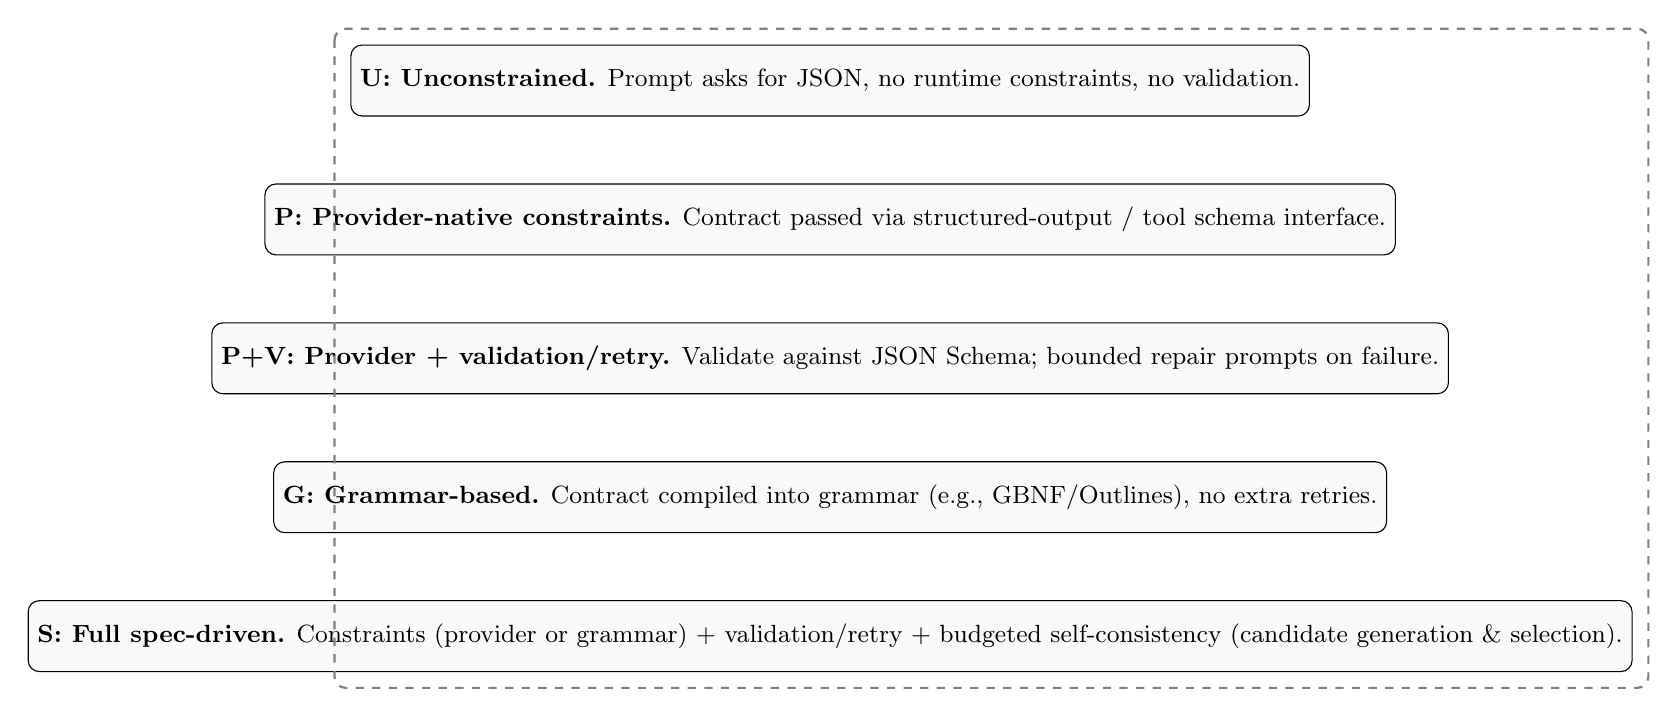
\begin{tikzpicture}[
    font=\small,
    node distance=0.85cm,
    layer/.style={draw, rounded corners, align=left, minimum width=0.9\linewidth, minimum height=0.9cm, fill=gray!5},
    title/.style={font=\bfseries},
]
\node[layer] (u) {\textbf{U: Unconstrained.} Prompt asks for JSON, no runtime constraints, no validation.};

\node[layer, below=of u] (p) {\textbf{P: Provider-native constraints.} Contract passed via structured-output / tool schema interface.};

\node[layer, below=of p] (pv) {\textbf{P+V: Provider + validation/retry.} Validate against JSON Schema; bounded repair prompts on failure.};

\node[layer, below=of pv] (g) {\textbf{G: Grammar-based.} Contract compiled into grammar (e.g., GBNF/Outlines), no extra retries.};

\node[layer, below=of g] (s) {\textbf{S: Full spec-driven.} Constraints (provider or grammar) + validation/retry + budgeted self-consistency (candidate generation \& selection).};

\draw[rounded corners, thick, dashed, gray]
    ($(u.north west)+(-0.2,0.2)$)
    rectangle
    ($(s.south east)+(0.2,-0.2)$);

\end{tikzpicture}
\caption{Configuration ladder used in experiments.
Each step adds one operational mechanism, enabling clean attribution of changes in structural correctness, faithfulness, stability, and tail latency.}
\label{fig:config-ladder}
\end{figure}

\paragraph{Shared decoding knobs.}
To ensure comparability, we fix the following unless explicitly swept:
temperature, top-$p$, max output tokens, and request formatting (system/prompt template).
When a backend supports \texttt{response\_format} or tool schemas, we pass the \emph{same} JSON Schema used by the validator.

\paragraph{Validation-and-retry budget.}
P+V and S apply bounded repair: if a response fails schema validation, the harness issues a \emph{structured repair prompt} that includes a compact error taxonomy (missing keys, type mismatch, enum violation) and requests a corrected JSON object.
We cap retries by a strict budget (e.g., 1--2 retries) and account for the full retry time in end-to-end latency.

\paragraph{Budgeted self-consistency.}
S optionally generates $k$ candidates (bounded by wall-clock and token budgets) and selects the final output using a criteria-weighted selector that prefers:
(i) schema validity,
(ii) higher task score proxies (when available),
(iii) higher faithfulness/support scores (for grounded tasks),
(iv) lower disagreement proxies (e.g., canonical JSON stability).
Candidate generation and selection are \emph{budgeted} so SLOs remain enforceable.

\begin{table}[t]
\centering
\small
\begin{tabular}{@{}lcccc@{}}
\toprule
\textbf{Config} & \textbf{Constraints} & \textbf{Validator} & \textbf{Retries} & \textbf{Self-consistency} \\
\midrule
U   & none & -- & 0 & 0 \\
P   & provider schema/tools & -- & 0 & 0 \\
P+V & provider schema/tools & JSON Schema & bounded & 0 \\
G   & grammar/regex constraints & -- & 0 & 0 \\
S   & provider or grammar & JSON Schema & bounded & bounded ($k_{\max}$, budgets) \\
\bottomrule
\end{tabular}
\caption{Compared configurations and which enforcement mechanisms are active.}
\label{tab:config-summary}
\end{table}

\subsection{Metrics and Reporting}
\label{sec:metrics-reporting}

\paragraph{Per-episode measurement.}
For each episode we compute the full metric vector from Section~\ref{sec:problem-metrics}:
\emph{structure} (parse + schema validity),
\emph{accuracy} (task-specific),
\emph{faithfulness} (atomic support and contradiction rate, where applicable),
\emph{tools/trajectory} (tool success and redundancy),
\emph{stability} (Disagreement@$k$ on repeated runs),
and \emph{latency/SLO} (end-to-end wall-clock, TTFT if available, Success@\slo).

\paragraph{Aggregation and uncertainty.}
We report means and rates per task family, and summarize latency with p50/\pninetyfive/\pninetynine.
For headline comparisons we additionally report 95\% confidence intervals via bootstrap resampling over episodes.
All plots (latency histograms, QPS frontiers, per-metric breakdowns) are exported from W\&B dashboards and included as static figures in the manuscript.

\paragraph{SLO accounting.}
Success@\slo is computed as an episode-level indicator that requires:
(i) passing all \emph{quality gates} defined in \texttt{criteria.yaml} (structure + task + faithfulness + tools + stability, as configured), and
(ii) meeting the latency constraint under the chosen budget.
This makes SLO compliance a \emph{joint} property of quality and responsiveness, matching production reality.

\begin{figure}[t]
\centering
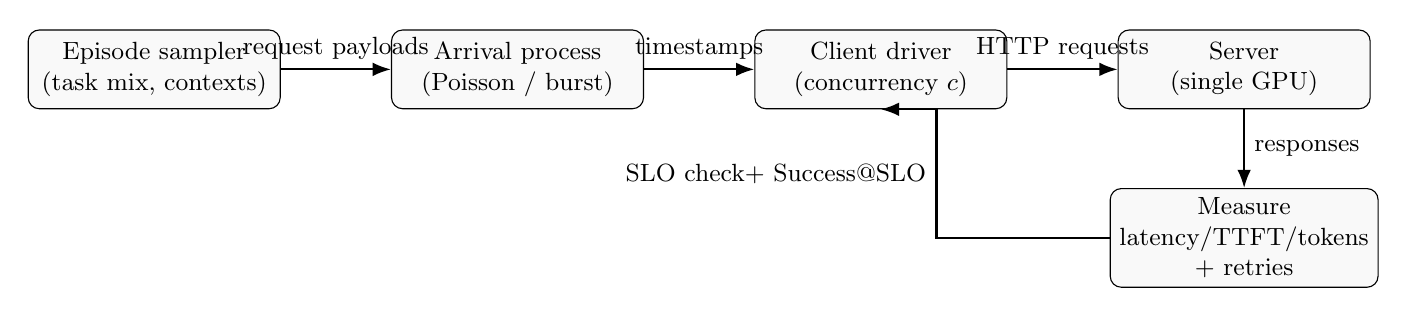
\begin{tikzpicture}[
    font=\small,
    node distance=1.0cm and 1.4cm,
    box/.style={draw, rounded corners, align=center, minimum width=3.2cm, minimum height=1.0cm, fill=gray!5},
    line/.style={-Latex, thick}
]
\node[box] (sampler) {Episode sampler\\ (task mix, contexts)};
\node[box, right=of sampler] (arrival) {Arrival process\\ (Poisson / burst)};
\node[box, right=of arrival] (client) {Client driver\\ (concurrency $c$)};
\node[box, right=of client] (server) {Server\\ (single GPU)};
\node[box, below=of server] (measure) {Measure\\ latency/TTFT/tokens\\ + retries};

\draw[line] (sampler) -- node[above]{request payloads} (arrival);
\draw[line] (arrival) -- node[above]{timestamps} (client);
\draw[line] (client) -- node[above]{HTTP requests} (server);
\draw[line] (server) -- node[right]{responses} (measure);
\draw[line] (measure.west) -- ++(-2.2,0) |- node[pos=0.25,left]{SLO check\\ + Success@\slo} (client.south);

\end{tikzpicture}
\caption{Latency/SLO experiment structure.
A sampler builds a realistic mixture of episodes; an arrival process generates timestamps; a concurrent client driver issues requests against a single-GPU server; and measurement includes \emph{all} retries/validation to reflect true downstream-usable latency.}
\label{fig:slo-harness}
\end{figure}

\subsection{Structural and Faithfulness Effects of Spec-Driven Decoding}
\label{sec:results-structure-faith}

Across all tasks, the most operationally important effect of constraints and validation is the removal of \emph{rare, catastrophic} structural failures:
invalid JSON, missing required keys, and type violations that break downstream code paths.
In practice, these failures are underrepresented by average-case quality metrics but dominate incident rates in production pipelines.

\paragraph{Structure.}
U (prompt-only) can achieve strong task metrics while still producing occasional malformed JSON or schema violations.
P improves structural adherence but remains dependent on backend implementation details.
P+V and S dominate on structure because explicit schema validation converts “silent” structural drift into actionable error codes, and bounded retries recover many fixable cases without human intervention.

\paragraph{Faithfulness.}
On grounded QA (T2), enforcing a structured explanation schema does \emph{not} automatically guarantee faithfulness; it merely forces the output to be parseable.
SpecSLOEval therefore treats faithfulness as a first-class family: S can use modest candidate generation to reduce contradiction rate by selecting outputs with higher support under the same contract, while still remaining budgeted under SLO constraints.

\subsection{Latency, SLOs, and Configuration Trade-offs}
\label{sec:results-slo}

Contract-first enforcement introduces overhead: validation, retries, and self-consistency add work that manifests primarily in the tail.
Our framework makes this explicit by reporting p95/p99 and Success@\slo jointly.

\paragraph{Representative latency snapshots.}
To anchor the discussion, we report two representative measurements from our current single-GPU baselines:

\begin{table}[t]
\centering
\small
\begin{tabular}{@{}lcccc@{}}
\toprule
\textbf{Setting} & \textbf{JSON valid} & \textbf{TTFT} & \textbf{\pninetyfive} & \textbf{\pninetynine} \\
\midrule
LM Studio baseline (structured + validation) & 100\% & $\approx$ 0.57s & $\approx$ 0.59s & $\approx$ 0.59s \\
Long-context GRPO snapshot (spec-driven) & 99.7\% & $\approx$ 1.88s & $\approx$ 3.10s & $\approx$ 3.14s \\
\bottomrule
\end{tabular}
\caption{Representative latency/structure snapshots (single RTX~4090).
Values are illustrative baselines from current runs; full frontiers are reported via QPS sweeps (Figure~\ref{fig:slo-harness}) and logged to W\&B.}
\label{tab:latency-snapshots}
\end{table}

\paragraph{Trade-off interpretation.}
U generally has the lowest raw latency but the highest risk of structural failures and brittle tool behavior.
P often sits between U and P+V on latency while improving parseability.
P+V typically adds small average overhead but reduces catastrophic failures, which often improves end-to-end system throughput in practice (fewer downstream retries/crashes).
S adds controllable overhead; its value is highest on tasks where correctness and faithfulness dominate and where modest candidate selection yields meaningfully better outputs per request.

\subsection{Backend and Model Comparisons}
\label{sec:results-backends}

Because SpecSLOEval is backend-agnostic, it enables apples-to-apples comparisons across runtimes and model sizes under the same contract and criteria gates.

\paragraph{Runtime effects.}
LM Studio, Ollama, and vLLM differ in batching policy, KV-cache strategy, and practical structured-output behavior.
These differences show up most clearly in \pninetyfive/\pninetynine and Success@\slo under QPS sweeps, where queueing and tail behavior dominate.

\paragraph{Model size effects.}
Larger models generally improve accuracy and grounded reasoning (T2) at the cost of latency and lower sustainable QPS under fixed SLOs.
The right choice is therefore workload- and SLO-dependent; SpecSLOEval’s configuration ladder (Figure~\ref{fig:config-ladder}) and frontier measurements make this trade-off explicit rather than anecdotal.

\subsection{Summary and Link to RL (P2)}
\label{sec:results-summary}

The experimental protocol in this section establishes a measurement surface that is operationally meaningful:
contract validity, task success, faithfulness, tool behavior, stability, and tail latency are measured together under a single criteria contract.
This is useful for \emph{static} selection of $(R,\delta,\mathcal{C})$ with frozen $\pi_\theta$ (P1), and it directly defines reward/cost components for \emph{constrained} optimization of $\theta$ (P2) using PPO/GRPO-style trainers and LoRA adapters.
In both cases, the core principle is the same: optimization should happen in the same metric space that production systems actually gate on.

\section{Discussion and Limitations}
\label{sec:discussion}

SpecSLOEval is motivated by a pragmatic observation: in production, an ``agent'' is evaluated as a \emph{service}, and services fail along dimensions that are not well-captured by single-number benchmark scores.
P1 intentionally targets the failure modes that most frequently break downstream systems on single-node deployments: malformed structured outputs, unfaithful or over-claimed statements relative to the available context, brittle tool trajectories, instability across repeated runs, and heavy-tailed latency that violates \pninetyfive/\pninetynine budgets~\citep{dean2013tail}.
This section clarifies what our framework covers well, what it does not (yet) cover, and what additional work is required to make contract-first, SLO-aware evaluation robust in high-stakes deployments and under policy optimization.

\subsection{Coverage of Production Failure Modes}

We designed the P1 suite to surface three classes of failures that commonly dominate operational risk:

\begin{enumerate}[leftmargin=12pt]
    \item \textbf{Structural failures:} malformed JSON, schema violations, and cross-field inconsistencies that crash or poison downstream consumers.
    \item \textbf{Faithfulness failures:} fluent but unsupported claims (especially numerical or trend errors) that cause incorrect decisions.
    \item \textbf{Latency failures:} tail latency spikes (\pninetyfive/\pninetynine) that collapse throughput and degrade perceived reliability~\citep{dean2013tail}.
\end{enumerate}

Figure~\ref{fig:coverage-map} summarizes our coverage at a glance and highlights the intentionally de-scoped regions. The central design stance is that \emph{structure and correctness are not optional}: ``fast but wrong'' is treated as a failure mode in most enterprise agent settings, unless the application is explicitly latency-dominant.

\begin{figure}[t]
    \centering
    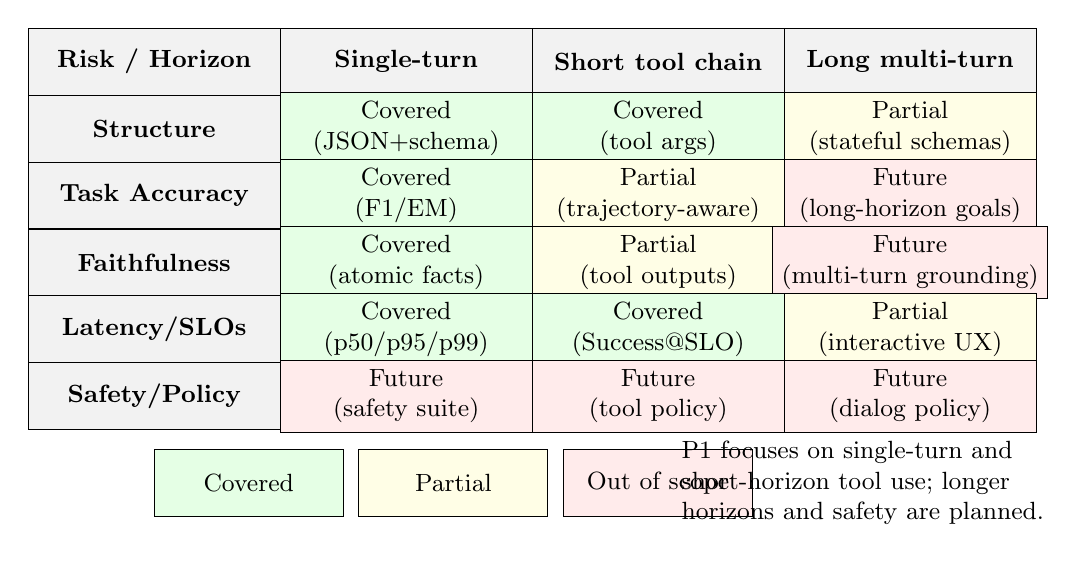
\begin{tikzpicture}[
        font=\small,
        cell/.style={draw, minimum width=3.2cm, minimum height=0.85cm, align=center},
        header/.style={draw, fill=gray!10, minimum width=3.2cm, minimum height=0.85cm, align=center, font=\small\bfseries},
        covered/.style={fill=green!10},
        partial/.style={fill=yellow!10},
        future/.style={fill=red!8},
        note/.style={align=left, font=\small}
    ]
    % Headers
    \node[header] (h0) at (0,0) {Risk / Horizon};
    \node[header] (h1) at (3.2,0) {Single-turn};
    \node[header] (h2) at (6.4,0) {Short tool chain};
    \node[header] (h3) at (9.6,0) {Long multi-turn};

    % Rows
    \node[header] (r1) at (0,-0.85) {Structure};
    \node[cell, covered] (r1c1) at (3.2,-0.85) {Covered\\ (JSON+schema)};
    \node[cell, covered] (r1c2) at (6.4,-0.85) {Covered\\ (tool args)};
    \node[cell, partial] (r1c3) at (9.6,-0.85) {Partial\\ (stateful schemas)};

    \node[header] (r2) at (0,-1.70) {Task Accuracy};
    \node[cell, covered] (r2c1) at (3.2,-1.70) {Covered\\ (F1/EM)};
    \node[cell, partial] (r2c2) at (6.4,-1.70) {Partial\\ (trajectory-aware)};
    \node[cell, future] (r2c3) at (9.6,-1.70) {Future\\ (long-horizon goals)};

    \node[header] (r3) at (0,-2.55) {Faithfulness};
    \node[cell, covered] (r3c1) at (3.2,-2.55) {Covered\\ (atomic facts)};
    \node[cell, partial] (r3c2) at (6.4,-2.55) {Partial\\ (tool outputs)};
    \node[cell, future] (r3c3) at (9.6,-2.55) {Future\\ (multi-turn grounding)};

    \node[header] (r4) at (0,-3.40) {Latency/SLOs};
    \node[cell, covered] (r4c1) at (3.2,-3.40) {Covered\\ (p50/p95/p99)};
    \node[cell, covered] (r4c2) at (6.4,-3.40) {Covered\\ (Success@\slo)};
    \node[cell, partial] (r4c3) at (9.6,-3.40) {Partial\\ (interactive UX)};

    \node[header] (r5) at (0,-4.25) {Safety/Policy};
    \node[cell, future] (r5c1) at (3.2,-4.25) {Future\\ (safety suite)};
    \node[cell, future] (r5c2) at (6.4,-4.25) {Future\\ (tool policy)};
    \node[cell, future] (r5c3) at (9.6,-4.25) {Future\\ (dialog policy)};

    % Legend
    \node[cell, covered, minimum width=2.4cm] (leg1) at (1.2,-5.35) {Covered};
    \node[cell, partial, minimum width=2.4cm] (leg2) at (3.8,-5.35) {Partial};
    \node[cell, future,  minimum width=2.4cm] (leg3) at (6.4,-5.35) {Out of scope};
    \node[note] at (9.0,-5.35) {P1 focuses on single-turn and\\ short-horizon tool use; longer\\ horizons and safety are planned.};

    \end{tikzpicture}
    \caption{Coverage map for SpecSLOEval (P1). Green cells indicate areas directly measured by the current test families; yellow indicates partial coverage (measured but with known gaps); red indicates areas that are intentionally de-scoped in P1 and require additional suites, datasets, and/or human evaluation.}
    \label{fig:coverage-map}
\end{figure}

\paragraph{What this means operationally.}
If your production risks are dominated by parsing errors, schema drift, faithless metric summaries, tool-call schema mistakes, and tail-latency collapse on a single node, SpecSLOEval is designed to be immediately useful.
If your risks are dominated by multi-turn negotiation, user experience, safety policy compliance, and long-horizon goal completion, then P1 should be treated as a foundation rather than a complete solution.

\subsection{Threats to Validity: What Can Go Wrong with the Measurement Itself}

Even a rigorous suite can mislead if the measurement apparatus does not reflect the deployed environment.
We therefore call out three practical threats to validity and how we mitigate them.

\paragraph{Construct validity (are we measuring the right thing?).}
Faithfulness scores are proxies (Section~\ref{sec:discussion-judge}), and tool-trajectory metrics can reward ``clean-looking'' behavior that does not correspond to actual user value.
We address this by (i) tying key pass/fail gates to hard operational constraints (schema validity, contradiction rate caps, Success@\slo), and (ii) encouraging teams to define application-specific metrics as additional families rather than forcing everything into a single scalar.

\paragraph{Internal validity (are the numbers reproducible?).}
Single-GPU latency distributions are sensitive to background processes, thermal throttling, and batcher dynamics.
We mitigate this by logging machine state metadata, pinning runtime versions, controlling seeds, and reporting quantiles over repeated runs rather than a single point estimate.

\paragraph{External validity (does offline $\widehat{W}$ predict production $W$?).}
Offline datasets can under-represent burstiness, unusual context lengths, rare tool failures, or user behaviors.
We mitigate this by explicitly parameterizing workload models, including burst tests, and recommending a promotion pipeline where offline gates are followed by staged canaries with the \emph{same} metrics computed online.

\subsection{Limitations of LLM-as-Judge Faithfulness}
\label{sec:discussion-judge}

Our use of LLM-as-judge faithfulness scoring follows RAGAS~\citep{es2023ragas} and atomic-fact evaluation~\citep{atomicFacts2024}, but inherits limitations common to judge-based approaches: prompt sensitivity, systematic blind spots (especially around numeric subtleties), and correlated failure modes when the judge and policy share training data or style biases.
Figure~\ref{fig:judge-pipeline} makes these failure points explicit.

\begin{figure}[t]
    \centering
    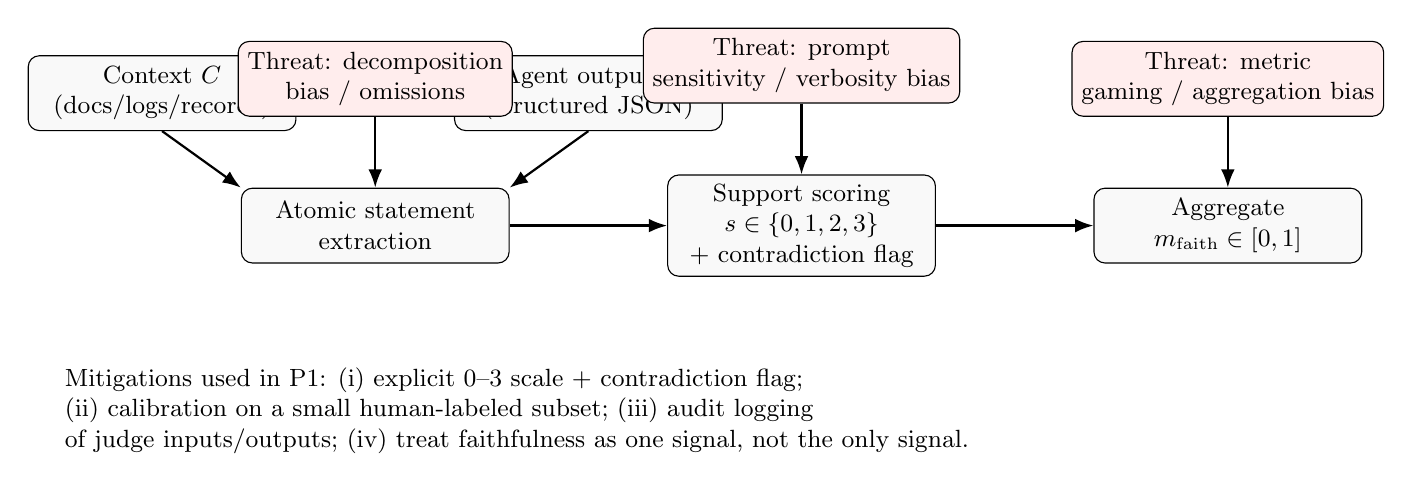
\begin{tikzpicture}[
        font=\small,
        box/.style={draw, rounded corners, align=center, minimum width=3.4cm, minimum height=0.95cm, fill=gray!5},
        warn/.style={draw, rounded corners, align=center, minimum width=3.4cm, minimum height=0.95cm, fill=red!7},
        line/.style={-Latex, thick},
        note/.style={align=left, font=\small}
    ]
    \node[box] (ctx) {Context $C$\\ (docs/logs/records)};
    \node[box, right=2.0cm of ctx] (ans) {Agent output $y$\\ (structured JSON)};
    \node[box, below=1.2cm of $(ctx)!0.5!(ans)$] (extract) {Atomic statement\\ extraction};
    \node[box, right=2.0cm of extract] (score) {Support scoring\\ $s\in\{0,1,2,3\}$\\ + contradiction flag};
    \node[box, right=2.0cm of score] (agg) {Aggregate\\ $m_{\text{faith}}\in[0,1]$};

    \draw[line] (ctx.south) -- (extract.north west);
    \draw[line] (ans.south) -- (extract.north east);
    \draw[line] (extract) -- (score);
    \draw[line] (score) -- (agg);

    % Threat callouts
    \node[warn, above=0.9cm of extract] (t1) {Threat: decomposition\\ bias / omissions};
    \node[warn, above=0.9cm of score] (t2) {Threat: prompt\\ sensitivity / verbosity bias};
    \node[warn, above=0.9cm of agg] (t3) {Threat: metric\\ gaming / aggregation bias};

    \draw[line] (t1.south) -- (extract.north);
    \draw[line] (t2.south) -- (score.north);
    \draw[line] (t3.south) -- (agg.north);

    \node[note, below=1.2cm of extract, xshift=1.8cm] {
        Mitigations used in P1: (i) explicit 0--3 scale + contradiction flag;\\
        (ii) calibration on a small human-labeled subset; (iii) audit logging\\
        of judge inputs/outputs; (iv) treat faithfulness as one signal, not the only signal.
    };

    \end{tikzpicture}
    \caption{Judge-based faithfulness pipeline and where bias can enter. Making these failure points explicit helps prevent ``metric overconfidence'' and informs mitigations such as calibration, auditing, and multi-signal gating.}
    \label{fig:judge-pipeline}
\end{figure}

\paragraph{Practical mitigation stance.}
In P1 we treat judge-based faithfulness as a \emph{high-leverage but imperfect} proxy:
it is valuable for regression testing and for shaping improvements, but it should not be used as the sole acceptance criterion in high-stakes domains.
For promotion decisions, we recommend (i) periodic human audits on stratified samples, (ii) cross-judge comparisons (two different judge models or prompts), and (iii) targeted, programmatic checks for numeric claims when contexts are machine-readable (tables/time series).

\subsection{Schema and Grammar Expressiveness}

We use JSON Schema and grammar constraints (e.g., GBNF) because they are portable across runtimes and naturally align with how downstream systems consume agent outputs.
The limitation is expressiveness: many real invariants are relational or temporal and cannot be expressed cleanly as local type constraints.

\paragraph{Implications for latency and correctness.}
When constraints cannot be enforced during decoding, they shift to post-hoc validation, increasing reliance on validation-and-retry and complicating worst-case latency bounds.
This motivates two extensions beyond P1:
(i) a richer invariant layer (e.g., executable validators with bounded cost) that is first-class in the contract model, and
(ii) better ``repair prompts'' and structured error taxonomies that make retries more reliable and less verbose.

\subsection{Single-GPU Focus and Deployment Generality}

P1 targets a single GPU (RTX~4090 class) or a laptop-class accelerator (Apple M-series).
This is a deliberate design point: many teams start here for privacy, cost predictability, and operational simplicity.
However, scaling out introduces new phenomena not present on a single node: cross-replica variability, queueing and routing effects, multi-tenant interference, and network-induced tail latency.

\paragraph{What transfers, and what does not.}
The metric families transfer cleanly: structure, accuracy, faithfulness, tool behavior, stability, and SLO adherence remain meaningful.
What changes is the \emph{system boundary} of the latency metric and the workload model: cluster-level routing and batching policies become part of the configuration surface $\delta$, and additional observability (queue wait time, replica selection, network time) becomes necessary to attribute tail events.

\subsection{RL Integration Scope and Reward-Gaming Risks}

We emphasize that the P1 metrics are designed to be reused as reward components and constraints in P2.
This tight coupling is powerful, but it creates predictable failure modes in optimization:

\begin{itemize}[leftmargin=12pt]
    \item \textbf{Reward hacking:} the policy learns to emit minimally valid but uninformative JSON to maximize structure metrics.
    \item \textbf{Judge overfitting:} the policy learns quirks of the faithfulness judge rather than improving genuine grounding.
    \item \textbf{Rare-case regressions:} average metrics improve while rare, high-impact cases get worse.
\end{itemize}

\paragraph{Mitigation plan for P2.}
P2 should (i) treat critical requirements as hard constraints (schema validity, contradiction rate caps, explicit SLO budgets), (ii) maintain a shadow ``audit set'' not used for reward to detect overfitting, and (iii) incorporate adversarial tests targeted to known failure modes (numeric trends, schema drift, tool argument edge cases).
Critically, RL promotion should be gated by the same acceptance criteria used for static selection, not by reward improvements alone.

\subsection{Human Factors and Operational Adoption}

Finally, the framework only matters if it can be owned by engineers and product stakeholders.
We therefore treat \texttt{criteria.yaml} as a versioned contract between teams: changes to what ``good'' means are explicit, reviewable, and auditable.
However, a full six-family suite can be overwhelming for early adopters.

A pragmatic adoption path is:
\begin{itemize}[leftmargin=12pt]
    \item \textbf{Starter pack:} structure + task accuracy + basic latency gates.
    \item \textbf{Risk-hardening:} add faithfulness and tool-trajectory tests for high-risk workflows.
    \item \textbf{Operational robustness:} add stability tests and bursty SLO workloads.
    \item \textbf{Optimization:} enable RL only after metrics are stable, calibrated, and understood by operators.
\end{itemize}

Table~\ref{tab:limitations} summarizes the main limitations and actionable mitigations/extensions.

\begin{table}[t]
\centering
\small
\begin{tabular}{p{3.2cm}p{5.0cm}p{6.8cm}}
\toprule
\textbf{Limitation} & \textbf{Why it matters} & \textbf{Mitigation / extension} \\
\midrule
LLM-as-judge bias & Faithfulness scores can drift, mis-rank outputs, or reward verbosity & Calibrate on human labels; log judge traces; use multiple judges/prompts; add programmatic numeric checks where possible \\
\addlinespace
Schema/grammar expressiveness & Many invariants are relational/temporal and cannot be enforced during decoding & Post-hoc validators with bounded cost; structured repair prompts; richer contract layer for cross-field rules \\
\addlinespace
Offline vs production mismatch & $\widehat{W}$ can under-sample bursts, long contexts, and tool failures & Parameterized workload models; burst tests; staged canaries computing the same metrics online \\
\addlinespace
Single-node assumptions & Cluster routing and queueing affect tail latency and consistency & Expand observability; treat scheduling/routing as part of $\delta$; introduce per-component latency attribution \\
\addlinespace
RL reward gaming & Optimizing metrics can create degenerate behavior and judge overfitting & Hard constraints, audit sets, adversarial suites, and human gates for promotion \\
\bottomrule
\end{tabular}
\caption{Key limitations of the P1 framework and concrete mitigations/extensions that preserve the contract-first, SLO-aware philosophy.}
\label{tab:limitations}
\end{table}

\paragraph{Summary.}
P1 establishes a measurement regime that is actionable for single-GPU deployments and that directly targets production-grade failure modes: structural validity, faithfulness, tool reliability, stability, and tail-latency SLOs.
Its central limitations are predictable (judge bias, schema expressiveness, horizon length, and safety), and we have made them explicit to avoid over-claiming.
P2 builds on this foundation by using the same metrics as rewards and constraints while explicitly guarding against reward gaming and evaluator overfitting.


\section{Discussion and Limitations}
\label{sec:discussion}

The results and infrastructure described so far argue for a simple premise:
\emph{deployable} LLM agents must be treated as contract-bound services with explicit SLOs, not as free-form text generators.
SpecSLOEval makes this premise operational by combining (i) contract-first decoding and validation, (ii) multi-family evaluation metrics, and (iii) tail-latency aware SLO accounting in a single harness.
This section clarifies what failure modes that framework covers well today, what it does not (yet) cover, and which engineering and research risks remain when moving from offline evaluation to real production.

\subsection{Real-World Failure Modes and Coverage}

We intentionally center three failure classes that repeatedly show up in commercial deployments (analytics/BI agents, support automation, workflow engines, adtech orchestration, and internal copilots):

\begin{enumerate}[leftmargin=12pt]
    \item \textbf{Structural failures (integration risk).}
    Malformed JSON, schema violations, missing required fields, and type mismatches are ``small'' model mistakes that can hard-fail downstream systems (ETL, dashboards, workflow routers) and create brittle, hard-to-debug incidents.

    \item \textbf{Faithfulness failures (decision risk).}
    Fluent but unsupported claims about metrics, trends, entities, or actions are often worse than slow answers: they can trigger incorrect business decisions, mis-route tickets, or silently corrupt data products.

    \item \textbf{Latency failures (operational risk).}
    Heavy-tailed latency (p95/p99 spikes) degrades perceived reliability, collapses throughput under burst load, and breaks user trust even when average latency looks acceptable.
\end{enumerate}

SpecSLOEval's current ``P1'' scope is deliberately biased toward these risks.
Figure~\ref{fig:coverage-map} makes the boundary explicit: we measure and gate the core reliability axis (structure, correctness, faithfulness, tool behavior, stability, SLOs), while leaving several important dimensions as explicit extensions rather than pretending to solve them implicitly.

\begin{figure}[t]
\centering
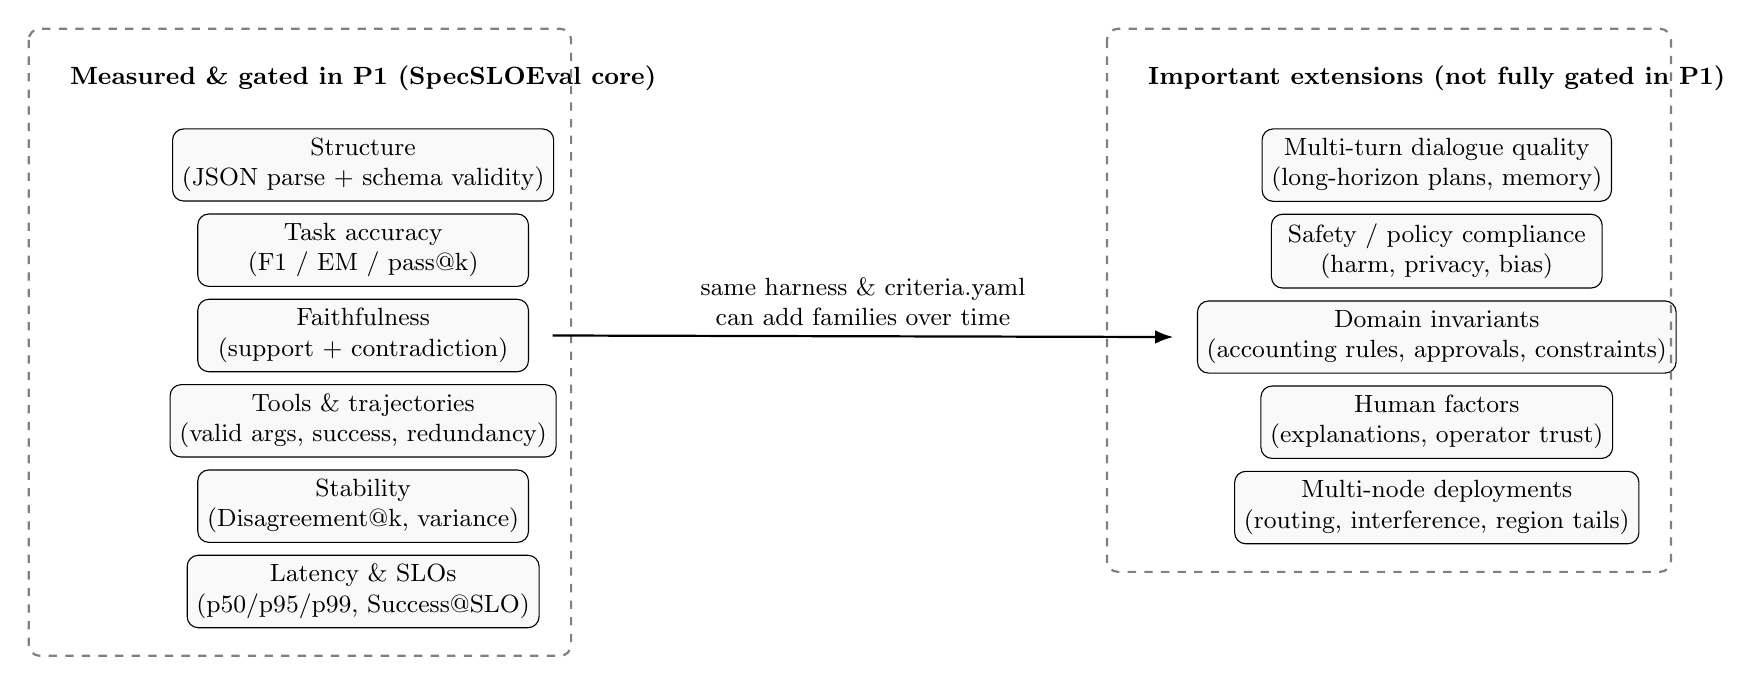
\begin{tikzpicture}[
    font=\small,
    box/.style={draw, rounded corners, align=center, minimum width=4.2cm, minimum height=0.9cm, fill=gray!5},
    title/.style={font=\small\bfseries},
    line/.style={-Latex, thick}
]
% Titles
\node[title] (tin) {Measured \& gated in P1 (SpecSLOEval core)};
\node[title, right=6.0cm of tin] (tout) {Important extensions (not fully gated in P1)};

% Left column (in-scope)
\node[box, below=0.35cm of tin] (c1) {Structure\\(JSON parse + schema validity)};
\node[box, below=0.15cm of c1]  (c2) {Task accuracy\\(F1 / EM / pass@k)};
\node[box, below=0.15cm of c2]  (c3) {Faithfulness\\(support + contradiction)};
\node[box, below=0.15cm of c3]  (c4) {Tools \& trajectories\\(valid args, success, redundancy)};
\node[box, below=0.15cm of c4]  (c5) {Stability\\(Disagreement@k, variance)};
\node[box, below=0.15cm of c5]  (c6) {Latency \& SLOs\\(p50/p95/p99, Success@\slo)};

% Right column (extensions)
\node[box, below=0.35cm of tout] (e1) {Multi-turn dialogue quality\\(long-horizon plans, memory)};
\node[box, below=0.15cm of e1]   (e2) {Safety / policy compliance\\(harm, privacy, bias)};
\node[box, below=0.15cm of e2]   (e3) {Domain invariants\\(accounting rules, approvals, constraints)};
\node[box, below=0.15cm of e3]   (e4) {Human factors\\(explanations, operator trust)};
\node[box, below=0.15cm of e4]   (e5) {Multi-node deployments\\(routing, interference, region tails)};

% Dashed group boxes
\draw[rounded corners, thick, dashed, gray]
    ($(tin.north west)+(-0.4,0.35)$)
    rectangle
    ($(c6.south east)+(0.4,-0.35)$);

\draw[rounded corners, thick, dashed, gray]
    ($(tout.north west)+(-0.4,0.35)$)
    rectangle
    ($(e5.south east)+(0.4,-0.35)$);

% Arrow between groups
\draw[line] ($(c3.east)+(0.3,0)$) -- node[above, align=center]{same harness \& criteria.yaml\\can add families over time} ($(e3.west)+(-0.3,0)$);

\end{tikzpicture}
\caption{Scope boundary.
SpecSLOEval (P1) gates the reliability-critical axis for contract-first agents (structure, correctness, faithfulness, tools, stability, and SLOs).
Several high-impact dimensions (multi-turn behavior, safety, domain invariants, human factors, multi-node effects) are explicit extensions rather than silently assumed.}
\label{fig:coverage-map}
\end{figure}

\subsection{Limitations of LLM-as-Judge Faithfulness}

Our faithfulness scoring follows the pragmatic ``LLM-as-judge'' pattern (RAGAS-style scoring and atomic-statement decomposition), but it must be treated as a \emph{measurement instrument} with known error modes rather than ground truth.

\paragraph{Key limitations.}
\begin{itemize}[leftmargin=12pt]
    \item \textbf{Prompt sensitivity and calibration drift.}
    Small changes to judge prompts or to the judge model can shift score distributions, which can silently break fixed thresholds if not versioned and monitored.

    \item \textbf{Systematic blind spots.}
    Judges often under-penalize subtle numeric misstatements (trend direction, percentage deltas, ranking errors) unless explicitly instructed and given strong negative examples.

    \item \textbf{Correlation and overfitting risk.}
    If the same (or closely related) model family is used for both policy and judge, or if RL directly optimizes the judge score, the system can overfit to judge idiosyncrasies instead of improving true groundedness.

    \item \textbf{Cost and latency coupling.}
    Judge calls add compute and can become part of the tail-latency story unless carefully budgeted or offloaded.
\end{itemize}

\paragraph{Operational mitigations we recommend.}
\begin{itemize}[leftmargin=12pt]
    \item \textbf{Version everything.}
    Judge model, judge prompt, and scoring code should be versioned and logged as artifacts alongside \texttt{criteria.yaml}.

    \item \textbf{Use ``hybrid checks'' where possible.}
    For numeric claims and schema-derived invariants, prefer deterministic validation (recomputing totals, verifying ordering, checking date logic) and treat the judge as a backstop for natural-language claims.

    \item \textbf{Calibrate with small human audits.}
    A lightweight labeled subset (even 50--200 examples per domain) is enough to sanity-check thresholds and detect drift.

    \item \textbf{Separate selection from evaluation.}
    If self-consistency uses a judge to select among candidates, evaluate final systems with a different prompt, different judge, or additional deterministic checks to reduce reward hacking.
\end{itemize}

\subsection{Schema and Grammar Expressiveness}

JSON Schema and grammar constraints are excellent for \emph{shape}, but limited for \emph{semantics}.
Many production contracts include invariants that are cross-field, temporal, or policy-dependent (e.g., accounting constraints, approval rules, permission-bound actions).

\paragraph{What works well today.}
\begin{itemize}[leftmargin=12pt]
    \item enforcing required/optional fields, types, enums, bounds, and simple array constraints at decode-time;
    \item eliminating catastrophic integration failures (non-JSON, missing keys, type mismatches);
    \item enabling stable downstream parsing and typed pipelines.
\end{itemize}

\paragraph{What remains hard.}
\begin{itemize}[leftmargin=12pt]
    \item cross-field equalities/inequalities and conservation laws (``must sum to 1'');
    \item conditional constraints (``if status=CLOSED then closed\_at exists and closed\_at $\le$ now'');
    \item business logic constraints (``discount $>$ 20\% requires approver and justification'').
\end{itemize}

\paragraph{Pragmatic design pattern.}
In production, the workable pattern is a \emph{two-layer contract}:
(1) schemas/grammars for syntactic shape and low-level types;
(2) post-hoc ``semantic validators'' for domain rules, with bounded repair loops.
This increases reliability but can introduce latency variance (validators and retries), which is why SpecSLOEval treats validation as part of end-to-end latency $L_\kappa(x)$ rather than an afterthought.

Table~\ref{tab:limitations-mitigations} summarizes these limitations and the mitigation strategies that keep the framework honest without claiming completeness.

\begin{table}[t]
\centering
\small
\begin{tabular}{@{}p{3.3cm}p{5.4cm}p{5.4cm}@{}}
\toprule
\textbf{Limitation} & \textbf{Why it matters} & \textbf{Mitigation in practice} \\
\midrule
Judge-based faithfulness noise &
Scores drift; subtle numeric errors slip through; RL can game judges &
Version judge+prompt; add deterministic checks; calibrate on small human subset; evaluate with alternative judge/prompt \\
\addlinespace
Schema/grammar expressiveness &
Cross-field and policy rules can't be encoded; invalid business actions may pass ``valid JSON'' &
Two-layer contracts: schema for shape + semantic validators; bounded repair loops; explicit error taxonomy \\
\addlinespace
Non-stationary workloads &
Traffic, context lengths, and tool latency shift; p95/p99 can regress without model changes &
Re-run SLO sweeps periodically; log workload summaries; include burst and long-context slices in CI \\
\addlinespace
Tool coupling and brittleness &
Tool schemas drift; downstream APIs change; agents fail with perfect language &
Tool mocks + contract tests; schema versioning; trajectory regression tests; fail-closed defaults \\
\addlinespace
Reward hacking in RL &
Agents optimize metrics, not business outcomes; can become uninformative but valid &
Hard gates for structure/faithfulness; holdout test sets not used for reward; periodic human audits \\
\bottomrule
\end{tabular}
\caption{Limitations and practical mitigations.
SpecSLOEval makes these risks explicit and measurable rather than implicit and surprising at deployment time.}
\label{tab:limitations-mitigations}
\end{table}

\subsection{Single-GPU Focus and Deployment Generality}

We target single-node deployments as a realistic and common baseline: one GPU (RTX~4090 class) or a laptop-class accelerator.
This choice forces the framework to confront tight compute budgets, queueing effects, and tail-latency sensitivity under burst load.
The metric families remain valid in larger deployments, but additional phenomena appear:

\begin{itemize}[leftmargin=12pt]
    \item cluster-level routing and interference (multi-tenant contention),
    \item network and cross-service latency components,
    \item regional tail effects (multi-region p95/p99),
    \item admission control and load shedding as first-class policies.
\end{itemize}

The current paper does not implement these cluster-level extensions, but the criteria-driven design intentionally keeps them additive: new SLO metrics and workload models can be introduced without changing the contract or scoring interfaces.

\subsection{RL Integration Scope and Risks}

SpecSLOEval's metrics are designed to be reused as reward components and constraints in P2, but the optimization surface introduces failure modes of its own.

\paragraph{Primary risks.}
\begin{itemize}[leftmargin=12pt]
    \item \textbf{Metric gaming:} produce trivially valid but low-information JSON to maximize structure scores.
    \item \textbf{Judge overfitting:} optimize the judge instead of truthfulness.
    \item \textbf{Rare-case regressions:} improve means while regressing on high-risk tails.
\end{itemize}

\paragraph{Guardrails we treat as non-negotiable.}
\begin{itemize}[leftmargin=12pt]
    \item strict gating order (structure/accuracy/faithfulness before stability and SLOs);
    \item fixed diagnostic sets not used for reward shaping;
    \item explicit ``fail-closed'' behaviors (timeouts and invalid outputs become structured errors, not free-form guesses);
    \item human-in-the-loop promotion checkpoints for model updates.
\end{itemize}

\subsection{Human Factors and Operational Adoption}

Even perfect metrics do not deploy themselves.
The central adoption challenge is to translate a multi-metric evaluation suite into a workflow that engineers and stakeholders trust.

Figure~\ref{fig:promotion-pipeline} depicts the promotion pipeline we assume in practice: offline evaluation produces a configuration candidate, strict gates prevent ``fast but wrong'' configurations from advancing, and canary deployments validate tail behavior under real traffic before broad rollout.

\begin{figure}[t]
\centering
\begin{tikzpicture}[
    font=\small,
    step/.style={draw, rounded corners, align=center, minimum width=3.1cm, minimum height=0.95cm, fill=gray!5},
    gate/.style={draw, rounded corners, align=center, minimum width=3.1cm, minimum height=0.95cm, fill=blue!5},
    line/.style={-Latex, thick},
    node distance=0.9cm and 1.0cm
]
\node[step] (logs) {Workload\\samples \& goldens};
\node[step, right=of logs] (offline) {Offline eval\\(SpecSLOEval)};
\node[gate, right=of offline] (gates) {Strict gates\\(criteria.yaml)};
\node[step, right=of gates] (canary) {Canary deploy\\(small traffic)};
\node[step, right=of canary] (monitor) {Monitor\\(tails + failures)};

\draw[line] (logs) -- (offline);
\draw[line] (offline) -- node[above]{metrics} (gates);
\draw[line] (gates) -- node[above]{pass} (canary);
\draw[line] (canary) -- node[above]{live tails} (monitor);

% Feedback loops
\draw[line] (monitor.south) .. controls +(0,-1.0) and +(0,-1.0) .. node[below, align=center]{regressions $\Rightarrow$ add tests\\or adjust budgets} (offline.south);
\draw[line] (monitor.north) .. controls +(0,1.0) and +(0,1.0) .. node[above, align=center]{promotion criteria\\\& dashboards} (gates.north);

\end{tikzpicture}
\caption{Operational promotion pipeline.
SpecSLOEval is designed to sit inside a practical release loop: offline tests and strict gating prevent brittle configurations from reaching production, while canaries validate tail-latency and rare-case behavior before full rollout.}
\label{fig:promotion-pipeline}
\end{figure}

In summary, SpecSLOEval is deliberately a \emph{reliability-first} skeleton.
It hardens the integration surface (contracts), measures the semantic risk surface (faithfulness), and forces tail behavior into the same scorecard as correctness.
P2 builds on this foundation by turning the same scorecard into a constrained optimization target, while preserving the guardrails above.

\section{Conclusion and Future Work}
\label{sec:conclusion}

This paper introduced SpecSLOEval: a spec-driven, SLO-aware framework for serving and evaluating LLM agents in realistic single-GPU deployments.
The core claim is operational:
\emph{if an agent is consumed by systems, it must behave like a contract-bound service.}
Accordingly, we treat the contract (JSON Schema / grammar) as the primary interface, and we evaluate agents with the same rigor used for production services: structural validity, task success, faithfulness to evidence, tool reliability, stability under re-runs, and tail-latency SLO compliance.

\paragraph{What P1 contributes.}
P1 establishes a baseline that practitioners can replicate and extend:

\begin{itemize}[leftmargin=12pt]
    \item \textbf{Contract-first agent serving.}
    A backend-agnostic contract layer that compiles to provider-native structured outputs and grammar-based constraints, and is hardened by bounded validation-and-retry and budgeted self-consistency under explicit token and wall-clock budgets.

    \item \textbf{A unified, auditable evaluation surface.}
    A single \texttt{criteria.yaml} defines metric families, gates, and weights, enabling consistent comparison across backends (LM Studio, Ollama, vLLM) and models, with per-episode logging for diagnosis and reproducibility.

    \item \textbf{A deployment-oriented measurement framing.}
    We treat p95/p99 and Success@\slo as first-class metrics alongside correctness and faithfulness, revealing trade-offs that are invisible when evaluation ends at average quality or JSON validity alone.
\end{itemize}

Figure~\ref{fig:specsloeval-stack} summarizes the end-to-end ``contract to deployment'' stack that P1 operationalizes.

\begin{figure}[t]
\centering
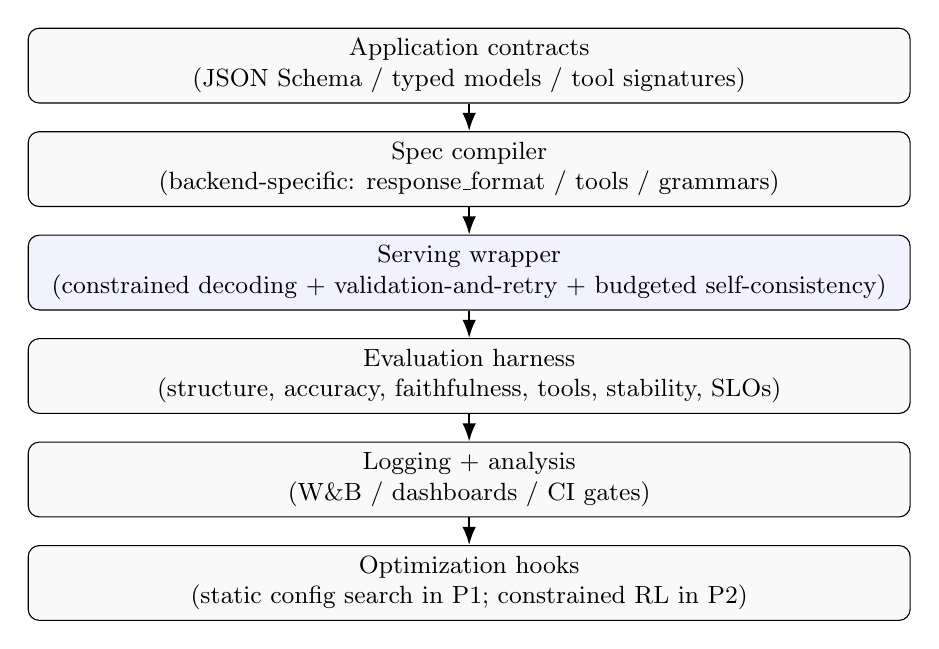
\begin{tikzpicture}[
    font=\small,
    layer/.style={draw, rounded corners, align=center, minimum width=11.2cm, minimum height=0.95cm, fill=gray!5},
    accent/.style={draw, rounded corners, align=center, minimum width=11.2cm, minimum height=0.95cm, fill=blue!5},
    line/.style={-Latex, thick},
    node distance=0.35cm
]
\node[layer]  (l1) {Application contracts\\(JSON Schema / typed models / tool signatures)};
\node[layer, below=of l1] (l2) {Spec compiler\\(backend-specific: response\_format / tools / grammars)};
\node[accent, below=of l2] (l3) {Serving wrapper\\(constrained decoding + validation-and-retry + budgeted self-consistency)};
\node[layer, below=of l3] (l4) {Evaluation harness\\(structure, accuracy, faithfulness, tools, stability, SLOs)};
\node[layer, below=of l4] (l5) {Logging + analysis\\(W\&B / dashboards / CI gates)};
\node[layer, below=of l5] (l6) {Optimization hooks\\(static config search in P1; constrained RL in P2)};

\draw[line] (l1) -- (l2);
\draw[line] (l2) -- (l3);
\draw[line] (l3) -- (l4);
\draw[line] (l4) -- (l5);
\draw[line] (l5) -- (l6);

\end{tikzpicture}
\caption{SpecSLOEval stack.
Contracts are compiled into backend constraints; serving is hardened by validation and budgeted self-consistency; evaluation computes a multi-family scorecard and enforces strict gates; the same scorecard supports CI and (in P2) constrained RL.}
\label{fig:specsloeval-stack}
\end{figure}

\paragraph{Future work.}
P1 is intentionally scoped and leaves several high-impact extensions:

\begin{itemize}[leftmargin=12pt]
    \item \textbf{Multi-turn and long-horizon workflows.}
    Extend test families to cover memory, planning under partial observability, escalation policies, and long-running tool workflows where latency composes over multiple steps.

    \item \textbf{Safety and policy as first-class families.}
    Add explicit safety/policy contracts (privacy constraints, sensitive data handling, refusal correctness, bias and fairness probes) with auditable thresholds in \texttt{criteria.yaml}.

    \item \textbf{SLO-aware reinforcement learning on a single GPU.}
    P2 will reuse the same metric surface as reward components and constraints (PPO/GRPO with LoRA adapters), emphasizing guardrails against reward hacking and tail regressions.

    \item \textbf{Richer contract languages.}
    Combine schema/grammar constraints with programmable semantic validators and domain-rule libraries so that contracts capture not only types but invariants (e.g., accounting identities, approval policies, campaign constraints).

    \item \textbf{Beyond single-node deployments.}
    Generalize workload models and SLO accounting to multi-node systems (routing, interference, multi-region tails) while preserving the contract-first interface and metric families.
\end{itemize}

The broader goal is standardization: a shared vocabulary and a portable, contract-first evaluation harness that makes agent reliability measurable and improvable.
SpecSLOEval is a step toward agents that are not only capable, but also \emph{structurally safe, evidence-faithful, stable under repetition, and predictable under tail latency} in the systems that depend on them.

\end{document}
